\documentclass[chaparabic,ceng,phd,12pt,oneandhalf,fivejury]{metu}
\usepackage{appendix}
\usepackage{longtable}
\usepackage[pdftex]{hyperref}
\usepackage[all]{hypcap}
\usepackage{todonotes}
\usepackage{graphicx}
\graphicspath{ {./images/} }
\usepackage[figuresright]{rotating}
\usepackage{xy} 
\usepackage{booktabs}
\usepackage{pifont}
\usepackage{color}
\usepackage{listings}
\usepackage{pdfpages}
\usepackage{array}
\usepackage{algorithm}
\usepackage{algorithmic}
\usepackage{float}
\usepackage{caption}
\usepackage{lastpage}
\usepackage{afterpage}
\usepackage{lipsum}
\usepackage{adjustbox}
\usepackage{rotating}

% \usepackage{graphicx}
\usepackage{amsmath,amssymb} % define this before the line numbering.
% \usepackage{ruler}
\usepackage{color}
% \usepackage{cite}
% \usepackage[utf8x]{inputenc}
% \usepackage{footnote}
% \makesavenoteenv{tabular}
% \makesavenoteenv{table}

\renewcommand{\sectionautorefname}{\S}
\renewcommand{\subsectionautorefname}{\S}

\newcommand{\norm}[1]{\left\lVert#1\right\rVert}

\captionsetup{belowskip=12pt,aboveskip=8pt}
\newcommand{\tab}{\hspace*{2em}}
\DeclareGraphicsExtensions{.pdf,.png,.jpg}


\usepackage{amsmath}
\usepackage{siunitx}
\usepackage{textcomp}
\usepackage{subcaption}


\usepackage{tikz}
\usepackage{mathtools}
% \usepackage{rotating}
%\PassOptionsToPackage{figuresright}{rotating}

\DeclarePairedDelimiter\ceil{\lceil}{\rceil}
\DeclarePairedDelimiter\floor{\lfloor}{\rfloor}


\newcommand{\EA}[1]{\textcolor{red}{[EA: #1]}}

% Name and Surname
\author{Merve Aydınlılar}
% Thesis Title English and Turkish
\title{Visual Similarity for HDR Images with Applications to Tone Mapping}
\turkishtitle{ODTÜ Tez Şablonu}

\date{Feb 2021}
 
% prof : Prof. Dr.
% assocprof : Assoc. Prof. Dr.
% assistprof : Assist. Prof. Dr.
% dr : Dr.
%
% Director of Institute
\director[prof]{Name Surname}
% Head of Department
\headofdept[prof]{Name Surname}
%
% Supervisor : English and Turkish
\supervisor[prof]{Ahmet Oğuz Akyüz}
% \turkishsupervisor{  } %if you will hard-code the academic title
%
% Affiliation of Supervisor in English and possibly in Turkish
\departmentofsupervisor{Computer Engineering, METU}

\cosupervisor[prof]{Sibel Tarı}
\departmentofcosupervisor{Computer Engineering, METU}
%
% Committee Members
% In general members are sorted according to their academic titles
%
% Proffesors (1)
% Associate Professors (2)
% Assistant Professors (3)
% Other (4)
% 
% IMPORTANT:  All affiliatons should fit in a single line
% If affiliation line is broken into two lines you should shorten the affiliation by using 
% abbrevations or any other means
%
% First committee member should be the chair of examining committee
% Typically the chair is one of the highest ranked committee members
% Ask your supervisor if you are not sure
\committeememberi[assistprof]{Name Surname}
\affiliationi{Computer Engineering, METU}
% Second committee member is always your supervisor
\committeememberii[assistprof]{Name Surname}
\affiliationii{Computer Engineering, METU}

% IMPORTANT: If you are Ph.D. student your co-supervisor can not be in your 
% examination committee.

% \def\@proftitlename{Prof. Dr.}\def\@tproftitlename{Prof. Dr.}
% \def\@assocproftitlename{Assoc. Prof. Dr.}\def\@tassocproftitlename{Doç. Dr.}
% \def\@assistproftitlename{Assist. Prof. Dr.}\def\@tassistproftitlename{Yrd. Doç. Dr.}
% \def\@drtitlename{Dr.}\def\@tdrtitlename{Dr.}

\committeememberiii[assistprof]{Name Surname}
\affiliationiii{Computer Engineering, Bilkent University}
% Fourth committee member
\committeememberiv[assistprof]{Gülşah Tümüklü Özyer}
\affiliationiv{Computer Engineering, Atatürk University}
% Fifth committee member
\committeememberv[assistprof]{Jüri}
\affiliationv{JüriBölüm, Ankara University}
%
% Keywords : English & Turkish, Comma seperated
\keywords{keywords, seperated, with, comma}
\anahtarklm{virgülle, ayrılmış, anahtar, kelimeler}
%
% Abstract in English
%
\abstract{
Assessing visual similarity for low dynamic range (LDR) images is an extensively studied
problem. Promising results are obtained when an image database is queried to find the images
containing a specific object of interest, a task known as exact matching. However, this problem
becomes more difficult if one needs approximate similarity, which is the task of determining
images that are merely visual similar to a query image. In this study, we aim to shed light on this
problem with an experimental approach. To this end, we first collect crowd-sourcing data
through a novel web-based experimental interface, in which the participants assess the visual
similarity of HDR images. We then collect a large number of features to assess how well they
correlate with the participants responses. We also include features computed by convolutional
neural networks, which are also proven to be successful in standard similarity tasks. We
compute the correlation of each feature with the crowdsourcing data, first in isolation, and then
merging multiple features by using different weights for each feature determined through a
metric learning approach. Based on the obtained results, we proposed a style-based tone
mapping algorithm that can successfully impart a user-defined style to various HDR images
determined to be similar with respect to our metric.
}
%
% Turkish Abstract
%
\oz{
Çok çeşitli amaçlarla kullanılmak üzere standard imgelerin benzerliğini belirleyen bir çok
algoritma bulunmasına rağmen HDR imgeler için yapılmış çalışma sayısı oldukça azdır.
Teknolojinin gelişmesiyle birlikte HDR imgelerin benzerliğinin objektif bir biçimde
değerlendirilmesi önem kazanacaktır. Bu sebeple, imgelerin benzerliklerini ölçmede etkili
olacağını düşündüğümüz, imgelerin alt ve orta seviye özelliklerini ve uzaklık metriklerini öne
sürüyoruz. Yaptığımız kullanıcı deneyi ile subjektif benzerlik skorları elde edilmiştir ve önerilen
özelliklerin bu skorlarla olan korelasyonu değerlendirilmiştir. Daha sonra, bu özelliklerin çeşitli
ağırlıklarla oluşturulan kombinasyonunun her bir özellikle tek tek elde edilen sonuçlardan daha
başarılı sonuç verdiği gözlenmiştir. Geliştirilen tekniğin bir uygulaması olarak HDR imgelerin
standard imgelere dönüştürülmesi probleminde imgeler arası benzerliğin kullanılmasının etkisi
gösterilmiştir. 
} 
%
% Dedication 
\dedication{Lorem ipsum dolor sit amet}
%
%
% Acknowledgements   
\acknowledgments{}

%
% End of Personal and Introductory  Information
%%%%%%%%%%%%%%%%%%%%%%%%%%%%%%%%%5
\begin{document}
% Preliminaries
\begin{preliminaries}
% If you are willing to use any custom stuff before Chapters, put it here
% Such as List of Abbreviations
% Check the abbreviations.tex for a template list of abbreviations

\begin{theglossary}{LONGESTABBRV}
\item[ABBREVIATIONS]
\item[1D] 1 Dimensional 
\item[2D] 2 Dimensional
\item[2AFC] 2 Alternative Forced Choice
\item[BF] Bileteral Filter
\item[CNN] Convolutional Neural Network
\item[DCNN] Deep Convolutional Neural Network
\item[EMD] Earth Mover's Distance
\item[HDR] High Dynamic Range
\item[HSV] Hue, Saturation, Value
\item[HVS] Human Visual System
\item[LDR] Low Dynamic Range
\item[MOS] Mean Opinion Scores
\item[SIFT] Scale-Invariant Feature Transform
\item[SURF] Speeded Up Robust Features
\item[TMO] Tone Mapping Operator
\item[UM] Unsharp Masking

\end{theglossary}

% End of Preliminaries
\end{preliminaries}
%   
% Latex content Goes Here 
% 
%

\setlength{\parindent}{0em}
\setlength{\parskip}{10pt}

% You can add as many chapters
% CHAPTER 1
\chapter{introduction}
\label{chp:b1}
With the developments in digital imaging, the means of producing digital images became widely available and this led to vast amount of images and diverse applications. Assessing visual similarity of images is an important task for various applications including image retrieval and indexing~\cite{liu2007survey}, classification and clustering~\cite{kleiman2016toward}, image editing and style transfer~\cite{rawat2018find}. Depending on the context of the application, image similarity might be defined differently and the developed techniques differ accordingly. Due to its importance, significant amount of research is dedicated to measuring image similarity. 

Unlike some computer vision tasks like depth estimation or object detection, image similarity does not have a ground truth. Typically, it is hard to estimate a certain degree of similarity between two images without a given context or other images to compare. The lack of ground truth makes the research of image similarity harder in two aspects, learning models from the ground truth data directly and measuring the performance of the proposed image similarity method reliably. This makes subjective experiments highly valuable for the image similarity research.

The need for High Dynamic Range (HDR) imaging was realized for the first time in computer graphics to deal with the requirements of physically accurate lighting simulation systems~\cite{glassner1995principles}. Such systems produced numerically unbounded pixel values, necessitating their storage in HDR file formats~\cite{ward1998rendering}. HDR images have typically been termed as ``scene-referred'' as opposed to ``display-referred'' -- a term used for Low Dynamic Range (LDR) images~\cite{Rein2010}. However, as display devices have traditionally been low dynamic range, displaying these images on LDR devices required an operation known as tone mapping~\cite{Tumb93,Ward97}. Numerous tone mapping operators (TMOs) have been developed in literature ranging from simple contrast adjustments to complex algorithms modeling the human visual system~\cite{Ferw96} and the properties of display devices~\cite{Mantiuk2008}. These operators are developed with different motivations and yielding with perceptually and statistically different images. Many methods have also been produced to create photographic HDR images of real-world scenes~\cite{Debe97}, including dynamic scenes~\cite{sen2012robust,kalantari2017deep}. Besides computer graphics, HDR imaging has many application areas including studying of fossils~\cite{theodor2009high}, cultural heritage and archaeology~\cite{happa2010high}, structural engineering~\cite{grinzato2009seismic}, architecture~\cite{cai2013high}, medical imaging~\cite{harifi2015efficient,rizzi2018visual}, forensics~\cite{brown2010forensic}, and automotive industry~\cite{wu2012fast}.

While the majority of the produced and stored images are standard images, HDR imaging offers to capture much wider luminance range, closer to the human eye, compared to standard LDR imaging. Currently, HDR video formats HDR10+~\cite{HDR10+} and Dolby Vision~\cite{chinnock2016dolby} are becoming the main HDR video standards and the number of HDR compatible commercial TVs, Blu-ray devices, gaming consoles and mobile devices supporting these video format standards is increasing. Besides, lately main streaming platforms like Amazon Prime Video and Netflix started serving HDR video content. These progress on the standardization and the developed devices will increase the demand in HDR content production very soon. Additionally, with the emerging technologies that require to exceed the human visual system limitations such as autonomous driving, HDR imaging gains more importance in safety critical computer vision applications.

%Until the HDR devices become the main standard, in order to display HDR images on standard displays, HDR images are mapped to low dynamic range, which is a process known as tone mapping. There are many tone mapping operators that    
%Despite the lack of native HDR sensors and commercially available HDR displays, the popularity of HDR imaging increases. 

Many research problems and applications are common to both HDR and LDR imaging. However, LDR images consist of 8 bit integers, whereas HDR images are represented with floating point data and if they have not been calibrated a single pixel intensity may refer to completely different illumination values on different scenes. Therefore, using the solutions and methods that are originally devised for standard LDR images may not be feasible for HDR images. 


\section{ Problem Definition}
Since image similarity is a perceptual phenomenon without ground truth, there are several studies that conducted human experiments. All these works, however, assume that the image is given in standard low dynamic range format where the brightness information is suitably quantized to match the dynamic range of traditional image display devices. Yet, growing number of applications utilize High Dynamic Range (HDR) images with unbounded brightness values. It may be argued that HDR images pose no extra challenges and approaches designed for LDR images may directly be used to assess visual similarity of HDR images as well. There are several counter-arguments, however. First, HDR images contain potentially uncalibrated floating point data and two images that have vastly different pixel values may actually be very similar to each other. Second, the richness of information in an HDR image, despite causing difficulties, may aid in similarity assessment. For example, pixel values corresponding to a bright light source can be much higher than that of a white reflecting surface in an HDR image, while the two objects are likely to map to similar intensities in an LDR image. Third, using a standard similarity measure for an HDR image requires tone mapping, a problem for which a multitude of algorithms, each with a number of parameters, exist~\cite{yeganeh2012objective}.

Hence, there is a need for investigating visual similarity for HDR images. This need is the motivation of this thesis where assessing visual similarity between two images is experimentally investigated. To this end, subjective human judgments using crowdsourcing is collected and features are evaluated by comparing them to human judgments. To our knowledge this thesis serves as the first rigorous attempt to evaluate how visual similarity can be assessed between HDR images. Using the findings from the perceptual study, a tone mapping methodology is proposed where tone mapping parameters are automatically computed to impart a certain user-defined style to a given HDR image using the similarity between this image and several calibration images that are used to create this style.

\section{Contributions and Outline of the Thesis}
The main motivation of this thesis is to investigate visual similarity for HDR images. In Chapter~\ref{chp:b2}, a review of HDR imaging and image similarity is given. The image features and the distance metrics used in the rest of the thesis are given in Chapter~\ref{chp:b3}.

The first contribution of this thesis is a tone mapping methodology, namely style-based tone mapping, that uses image similarity to automatically estimate tone mapping parameters from the tone mapping parameters of a set of given images to follow a certain style. This tone mapping operator is presented in detail in Chapter~\ref{chp:b4}.

%The improvements achieved by using the findings from the user study is also provided.

Due to the subjective nature of the image similarity problem, an experimental study that assesses visual similarity between HDR images is conducted. The second contribution of this thesis is the novel web-based interface for the user experiment and the collected data through crowd-sourcing. The experimental setup and the details about data gathering is given in Chapter~\ref{chp:b5}. The third contribution is the investigation of the agreement of various image features and the corresponding distance metrics to the collected user data. In addition, a combined feature is estimated using experiment data. The effect of the tone mapping operator is also presented by repeating the analysis on the images that are tone mapped with commonly used tone mapping operators. These analyses on the user experiment are also given in the same chapter. In Chapter~\ref{chp:b6}, two methods to improve the style-based tone mapping operator by using the results obtained through user experiment are presented.

Lastly, discussion about the findings and the results are given in Chapter~\ref{chp:b7} and the summary of the thesis, several limitations and future directions are given in Chapter~\ref{chp:b8}.







\chapter{Related Work}
\label{chp:b2}

\section{Image Similarity}
%paper_start
Traditionally, image similarity is measured by measuring the distance between hand crafted features extracted from each image. These hand crafted features include simple descriptors such as color/luminance histograms, or improved ideas, including histogram of oriented gradients~\cite{dalal2005histograms}. GIST~\cite{oliva2001modeling}, SIFT~\cite{lowe2004distinctive}, SURF~\cite{bay2006surf}. These features are compared using several types of distance metrics. Recently, deep convolutional neural networks (DCNNs) became the state of art for image classification. Starting with AlexNet~\cite{krizhevsky2012imagenet} and followed by deeper networks such as VGG~\cite{simonyan2014very}, GoogLeNet\cite{szegedy2015going}, and ResNet~\cite{he2016deep}, DCNNs started to perform near human level success for image classification. Their success lead to use feature vectors that have been obtained from DCNNs for image retrieval~\cite{wan2014deep,gordo2016deep}. Unlike previous approaches that are based on hand-crafted features, DCNNs learn the feature vector itself directly from the image. One major drawback of using
DCNNs is the need for using very large labeled datasets for training, which is difficult to obtain or not available at all for most problem domains. Transfer learning~\cite{yosinski2014transferable} aims to solve this problem by using pretrained networks on large scale datasets such as ImageNet~\cite{russakovsky2015imagenet}. The basic method is to give the images to the pre-trained network and use the output of the last fully connected layers as feature vectors~\cite{donahue2014decaf,wan2014deep} -- an approach that we also adopt in our work.

Visual similarity is a perceptual phenomenon without ground-truth data. This makes collecting data using crowdsourcing experiments valuable. Indeed, there are several crowdsourcing-based works~\cite{lun2015elements,saleh2015learning,kleiman2016toward} that address shape or style similarity problems and conduct user experiments to either derive or validate models.

Of most related to our work are two similarity studies that also employ subjective experiments. Among these, in Rogowitz et al.~\cite{rogowitz1998perceptual}, human participants are asked to judge image similarity using two different experiments: one involving printouts of images (called table scaling) and the other using a computer based comparison (called computer scaling). These results are compared with computational similarity approaches~\cite{frese1997methodology} and simple CIELAB histograms. It was found that both table and computer scaling yield similar results and color is a major factor influencing similarity for human observers.

In another study~\cite{neumann2006image}, user experiments are conducted to evaluate the relationship between an image-indexing system and perceived similarity in an LDR setting. The tested image indexing system is based on basic properties of early stages of human vision -- chromaticity, luminance, and texture. Two-alternative forced-choice (2AFC) method is used for all experiments. Three images are shown to the observer, the query image and two test images. Of these two images one image is called the target and the other the distractor. These images are selected based on the rankings obtained from the image-indexing system. Then the correlation between the users' preference and index rank is investigated. First, each index, chromaticity, luminance, and texture are calculated separately. From these indexes chromaticity is found to give the best results. Then for the second experiment, combinations of the indexes are evaluated. The combination of chromaticity and texture indices are found to give better results than chromaticity alone and the combination of all indices are found to give the best result.
%paper_end

\section{HDR Imaging}
The need for HDR imaging was realized for the first time in computer graphics to deal with the requirements of physically accurate lighting simulation systems~\cite{glassner1995principles}. Such systems produced numerically unbounded pixel values, necessitating their storage in HDR file formats~\cite{ward1998rendering}. HDR images have typically been termed as ``scene-referred'' as opposed to ``display-referred'' -- a term used for LDR images~\cite{Rein2010}. However, as display devices have traditionally been low dynamic range, displaying these images on LDR devices required an operation known as tone mapping~\cite{Tumb93,Ward97}. Numerous tone mapping operators (TMOs) have been developed in literature ranging from simple contrast adjustments to complex algorithms modeling the human visual system~\cite{Ferw96} and the properties of display devices~\cite{Mantiuk2008}. Many methods have also been produced to create photographic HDR images of real-world scenes~\cite{Debe97}, including dynamic scenes~\cite{sen2012robust,kalantari2017deep}.

While HDR imaging has always been an active field of research, recent developments in HDR imaging~\cite{Rein2010,Banterle2011,chalmers2016high}, in particular those pertaining to HDR image and video capture~\cite{tocci2011versatile,froehlich2014creating} and display systems~\cite{seetzen2004high} to allow direct rendition of HDR images will likely make HDR images more ubiquitous in the near future. Consequently, we believe that assessing visual similarity of HDR images will also become an important problem.

As mentioned above, although visual image similarity is an extensively studied subject~\cite{liu2007survey}, to our knowledge there is no study that directly addresses this problem for HDR images. Thus, understanding the nature of image similarity for HDR images and developing an objective similarity measure is the primary goal of this paper. 
%paper_end

\subsection{Tonemapping}

\section{Features}
\label{sec:features}
%paper
In this study, five kinds of features are used to model HDR images: color, luminance, texture, GIST, and DCNN features. Table \ref{tab:table_feature} lists these features together with their representations and the distance metric used for each feature. The following sections outline the details of these features and the corresponding distance metrics.

\begin{table}[h!]
\caption{HDR Image features and distances}
\centering
\begin{tabular}{c|c|c}
\label{tab:table_feature}
\textbf{Feature} & \textbf{Model} & \textbf{Distance Metric}\\
\hline
Color  & 2D chromaticity histogram & Earth Mover's Distance (EMD) \\
Luminance  & 1D (relative) luminance histogram & EMD \\
Texture  & Histograms of gradients & EMD \\
GIST  & Feature vector & Cosine distance \\
VGG16/VGG19 - fc6 & Fused fc6 layer & Cosine distance  \\
VGG16/VGG19 - fc7 & Fused fc7 layer & Cosine distance
\end{tabular}
\end{table}

%paper
\subsection{Color}
%paper
Since the early days of the image similarity research, color has been used as one of the most discriminative cues~\cite{neumann2006image}. In this study,  we used the $a$ and $b$ channels of the CIELAB color space~\cite{iso201111664} to represent chromaticity information. This is an opponent color space, where the $a$ channel represents red/green opponent colors and the $b$ channel yellow/blue opponent colors. We used a 2D chromaticity histogram to represent the distribution of colors in a given image. Each dimension contained $15$ bins for a total of $225$ bins.  Figure~\ref{fig:hists} shows this histogram for the Mason Lake image from the
dataset~\cite{fairchild2007hdr}.

\begin{figure}
\centering
\caption{Sample image (left), 2D histogram (right).}
\label{fig:hists}
\begin{tabular}{c c}
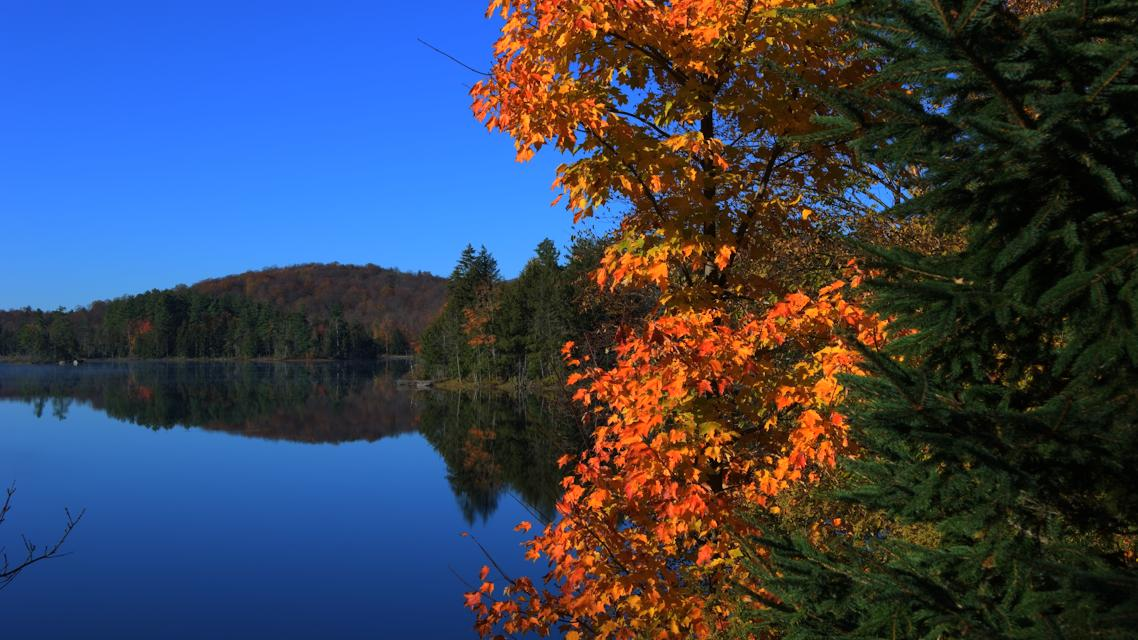
\includegraphics[height=1.8in]{figures/chapter2/MasonLake.jpg} &
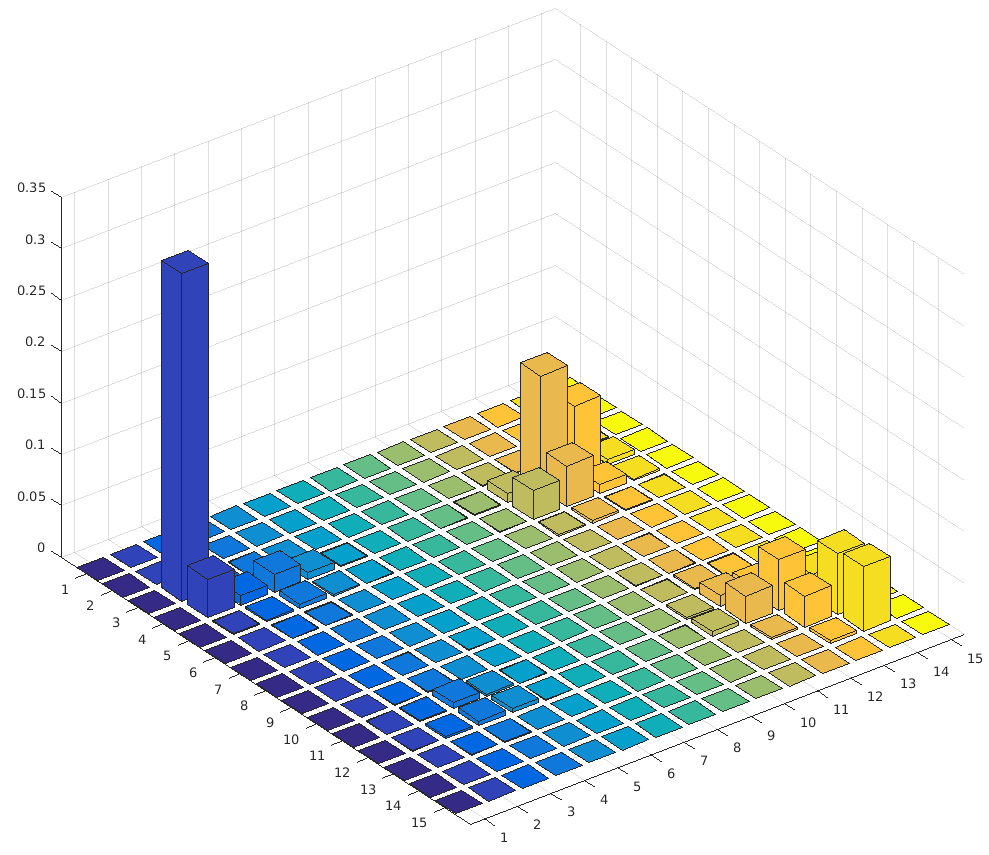
\includegraphics[height=1.8in]{figures/chapter2/57_histab.png}

\end{tabular}
\end{figure}

%paper
\subsection{Texture}
%paper
Texture is the second most used feature for content based image retrieval systems after chromatic features.  This feature is especially helpful for discriminating images that have similar color but different spatial characteristics such as blue sky and sea or sand and buildings.  To represent the texture information we used histogram of gradient magnitudes~\cite{sharma2015histogram}.
%paper
\subsection{Luminance}
%paper
The main difference between an HDR and an LDR image is the much wider range of luminance distribution for the former. A single HDR image may contain very low luminances corresponding to highly shadowed regions as well as very high luminances corresponding to bright highlights. Therefore, we hypothesized that the luminance distribution of an HDR image may be an important cue for visual similarity. The luminance distribution is modeled using a 1D (relative) luminance histogram with $50$ bins.
%paper
\subsection{GIST Features}
%paper
The GIST descriptor~\cite{oliva2001modeling} aims to represent the dominant spatial structure of a scene by using low level multi-scale representations. This descriptor defines the scene as a whole rather than focusing on individual objects or regions. Discriminative properties of a scene are listed as naturalness, openness, roughness, expansion, and ruggedness. The class of a scene, e.g., man-made, natural, indoor, outdoor, etc., is determined by these properties.

The procedure for extracting GIST descriptors consists of applying Gabor filters that are scaled and orientated differently to the input image, dividing the filter response map into a grid in order to have spatial information, averaging the filter response in each grid, and concatenating the results to obtain the final feature vector, i.e. the GIST descriptor.

%paper
\subsection{Deeply Learned Features}
%paper
Recently, DCNNs have started to dominate object recognition and image classification tasks, achieving near human success rates~\cite{krizhevsky2012imagenet,simon14,zhou2017scene}. These models are trained with large prelabeled datasets and develop a hierarchical model that becomes more aware of the content of the image rather than the underlying pixel values. To our knowledge currently there is no DCNN model that is trained on HDR images for the purpose of image indexing, scene classification, or visual similarity tasks.
Furthermore, there is no prelabeled large HDR image dataset to use for training a DCNN model from scratch. Therefore in this study, we used transfer learning method to employ pretrained DCNNs for our perceptual
similarity problem. 

For feature extraction, pretrained AlexNet~\cite{krizhevsky2012imagenet} and two variants of VGG networks, VGG16 and VGG19, are used~\cite{simon14}. All networks are trained on the ImageNet~\cite{russakovsky2015imagenet} dataset, but we also evaluated their performance when trained using
different datasets. For transfer learning, the last fully connected layer, which contains classification outputs, is removed and the remaining $4096$ dimensional two fully connected layers, \textbf{fc6} and \textbf{fc7}, are used as feature vectors. As suggested by Simonyan and Zisserman~\cite{simonyan2014very}, the results obtained from VGG16 and VGG19 are fused (by taking an average) and it is observed that
the fused version performs better than both VGG16 and VGG19. The distance between the feature vectors are calculated using cosine distance, which is a commonly used distance metric for deep learning features. 
%paper
\section{Distance Metrics}
%paper
The use of a proper distance metric is as important as the features themselves. Each feature representation
may require a different distance metric. In this section, we briefly describe the definitions and properties of the dissimilarity measures that we used for different types of features.
%paper
\subsection{Euclidean Distance}
%paper
The Euclidean distance between two histograms p and q is calculated as:
\begin{equation}
dist_{euc}(p,q) = \sqrt{\sum_i(p_i-q_i)^2},
\end{equation}
where i is the bin index. In general, dissimilarity obtained by Euclidean distance for histograms is not satisfactory as it does not take bin proximity into account.
%paper
\subsection{Bhattacharyya Distance}
%paper
Bhattacharyya distance~\cite{bhattacharyya1946measure} measures the overlap between two distributions. If p and q are two histograms, it can be calculated as:
\begin{equation}
dist_{bhat}(p,q) = -\ln \left( \sum_i \sqrt{p_i.q_i} \right).
\end{equation}

For our HDR similarity problem Bhattacharyya distance gives slightly better results than Euclidean distance. However, it also suffers from the same problem that the proximity of the bins is not taken into account.
%paper
\subsection{Earth Mover’s Distance}
%paper
Earth Mover’s Distance (EMD) is a dissimilarity metric commonly used for image the retrieval problems~\cite{rubner2000earth}. EMD aims to capture the perceptual similarity between two distributions by calculating the minimal cost of transforming one distribution to the other. Unlike the other dissimilarity metrics, EMD can be calculated for varying-size partitions of the data, called signatures.
Signatures consist of dominant clusters of the data, represented as $si = (m_i, w_i)$ pairs where mi is the cluster center and $w_i$ is the size of the cluster. EMD does not require the signatures to have the same number of clusters – ground distances between cluster centers are sufficient. Histograms are signatures with bin centers corresponding to cluster centers, mi, and normalized bin values to weights, $w_i$.

The total amount of work to transform distribution
p to q with flow f is:
\begin{equation}
WORK(P,Q,F) = \sum_i^m \sum_j^n d_{ij}f_{ij}, 
\end{equation}
where dij is the ground distance between cluster centers i and j. The optimal flow f that results with the minimum work, can be found by any linear optimization algorithm. When f is calculated, the EMD between p and q is defined as:
\begin{equation}
EMD(p,q) = {{\sum \sum d_{ij}f_{ij}}\over{\sum \sum f_{ij}}}.
\end{equation}
In our problem, bin centers correspond to color values
(ab values in the CIELAB space) and ground distances
are calculated as Euclidean because of the perceptual
uniformity of the CIELAB color space.

Figure \ref{fig:sim_comp} compares the effect of these three distance
metrics for a sample image from the dataset. The image
on the first column is the query image, and in each row,
the most similar five images from the dataset are shown.
The distance metric used in first row is Euclidean, the
second row is Bhattacharyya, and the last row is the
EMD. It can be argued that more similar images are
found using the EMD metric.

\begin{figure} 
\centering
\caption{A comparison of dissimilarity metrics for histogram-based features. The leftmost image is the query image, the most similar five images from the dataset are shown in each row: Euclidean distance (first row), Bhattacharyya distance (second row), Earth Mover’s distance (third row).}
\label{fig:sim_comp}
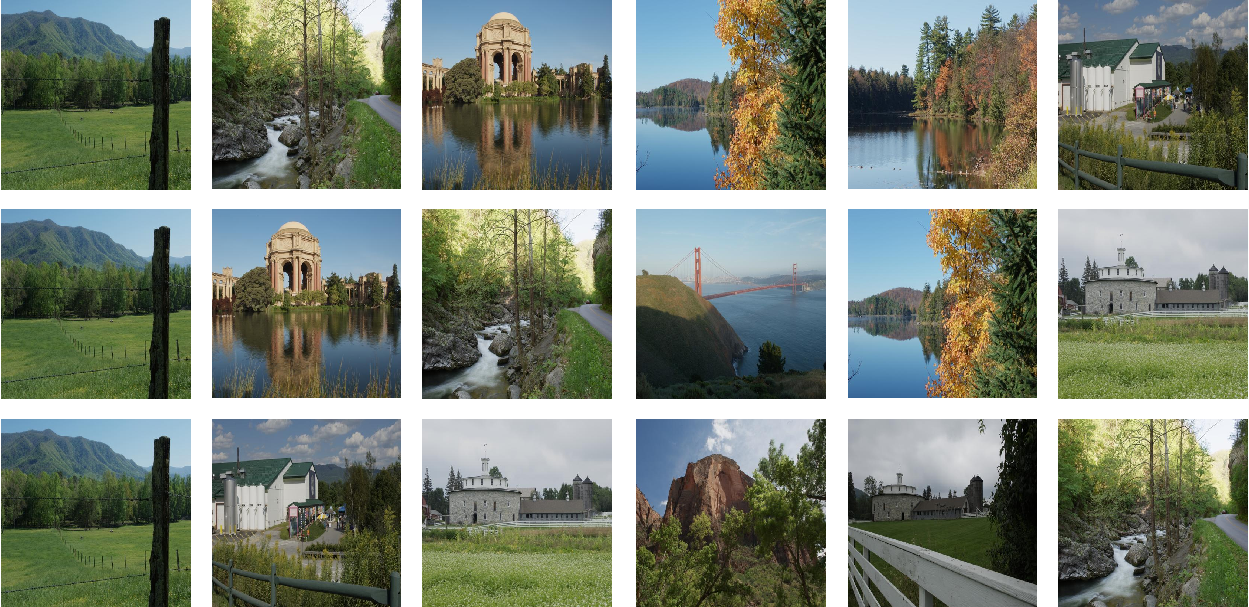
\includegraphics[width=\textwidth]{figures/chapter2/16sims.png}
\vspace{10pt}
\end{figure}

%paper
\subsection{Cosine Similarity}
%paper
Cosine distance between two vectors $p$ and $q$ is calculated as:
\begin{equation}
dist_{cosine}(p,q) = 1 - {{\sum_{i=1}^{n}p_{i}q_{i}} \over {\sqrt{\sum_{i=1}^{n}p_{i}^2}} \sqrt{\sum_{i=1}^{n}q_{i}^2}} 
\end{equation}
Cosine distance is a widely used distance metric for deep representations. In this study, we used cosine distance for calculating the distances between CNN feature vectors and GIST features.
%paper

























\chapter{User Study}
\label{chp:b3}

\section{Dataset}
%paper
The set of images used in visual similarity experiments should be sufficiently diverse. Although such datasets exists for LDR images, there is no specific similarity dataset for HDR images. However, there exists HDR image datasets that were created for various purposes and by different authors. We therefore decided to select 100 HDR images from various such sources to present observers with a diverse set of images2. The used datasets were: Fairchild’s HDR Photographic Survey [12], HDR-Eye [37], DEIMOS [25], Empa HDR Image Database [1], and pfstools HDR Image Gallery [32]. Thumbnails for the used images are shown in Figure \ref{fig:dataset}.

\begin{figure}
\begin{center}
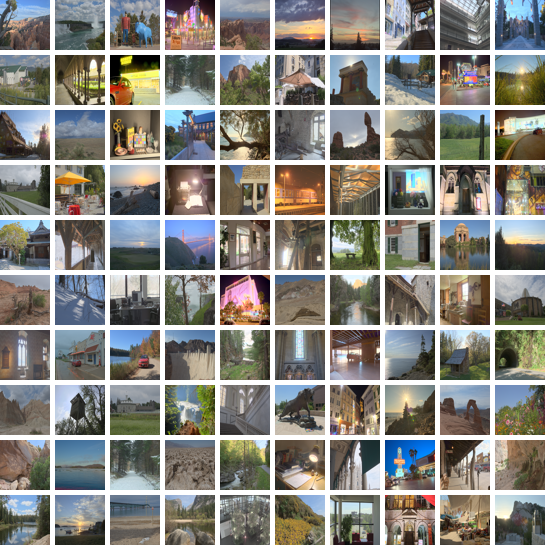
\includegraphics[width=\textwidth]{figures/chapter3/dataset.png}
\caption{HDR images used in the visual similarity experiments.
%paper
}
\label{fig:dataset}
\end{center}
\end{figure}
%paper
\section{Experiment Setting}
%paper
To measure perceptual similarity between HDR images, we conducted a 2AFC experiment. The experiment is publicly available\footnote{http://user.ceng.metu.edu.tr/~merve/userstudy/}. As we needed a large number of responses, we designed a web-based interface to collect crowdsourcing data. We used the HDRHTML technique [34] for visualizing HDR images on web browsers. This technique uses a windowing approach to select a desired exposure range from the HDR image, which is indicated by a slider set by the user. By dynamically adjusting the position of the slider, the user can efficiently view the entire exposure range contained within the HDR image. These sliders are normally overlayed with the image histogram. We removed this overlay to prevent the image histogram from affecting the observers’ decisions. Figure \ref{fig:experiment} shows a sample trial from the experiment. An HDR reference image was shown at the top and two HDR test images were shown at the bottom. The sliders, which were mandatory to be adjusted, allowed all images to be inspected at different exposure levels.

\begin{figure}
\begin{center}
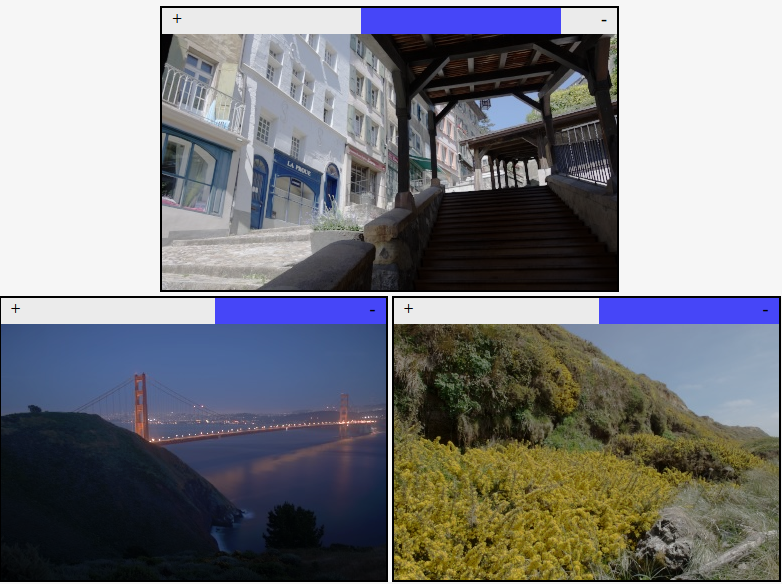
\includegraphics[width=\textwidth]{figures/chapter3/experiment.png}
\caption{EA sample trial from the experiment. The observers were asked to choose the most similar image to the reference image (top) from the test images (bottom). All images could be examined at different exposure levels by adjusting their sliders.
%paper
}
\label{fig:experiment}
\end{center}
\end{figure}

In each experimental session, 33 such image triplets were displayed to the observers. Thus, an experimental session consisted of 33 trials. In each trial, the observers were asked to choose which of the two test images was visually more similar to the reference image. Here it is important to note that we did not ask users
to decide for a specific type of similarity such as object, color, etc. By intentionally leaving the definition of visual similarity vague, we hoped to achieve a range of responses, which in overall, would converge to a common sense understanding for similarity. All trials, except for the verification ones, were generated randomly from the dataset during the runtime of the experiment. Three of these triplets were used for verification. They contained an obviously similar reference and test image pair to evaluate the reliability of an observer. If an observer failed to provide the correct answer even for one of these trials, his or her data was discarded as being unreliable. These trials were distributed evenly across the experiment to ensure that observers were attentive throughout. Before the experiment began, observers were informed about their task and the expected duration of the experiment, which was at most 20 minutes at a normal pace. During the experiment, observers were required to use the exposure sliders for each image before they made selection. Image selection was done by clicking on one of the test images. The selection was indicated using a green border around the selected image. Observers could change their selection until they pressed the “Next” button. The progress of an observer was indicated using a small progress bar at the bottom center of the screen. At the end of the experiment, observers were informed with a final page confirming the conclusion of the experiment and were presented with unique session ids. They were required to enter this id to the crowdsourcing platform to verify that they have finished the experiment.
%paper
\section{Data Collection}
%paper
In order to reach as many people as possible, the experiment was published at Microworkers crowdsourcing platform3. The number of payed users that participated in the experiment through this platform was 801. For each completed experiment 0.3\$ were paid.

Among these, 165 sessions were discarded due to incorrect responses given to the verification trials. Age, gender, and familiarity with computer graphics/image processing distribution of the participants are shown in Figure \ref{fig:age_gender_cgi}.

\begin{figure}
\begin{center}
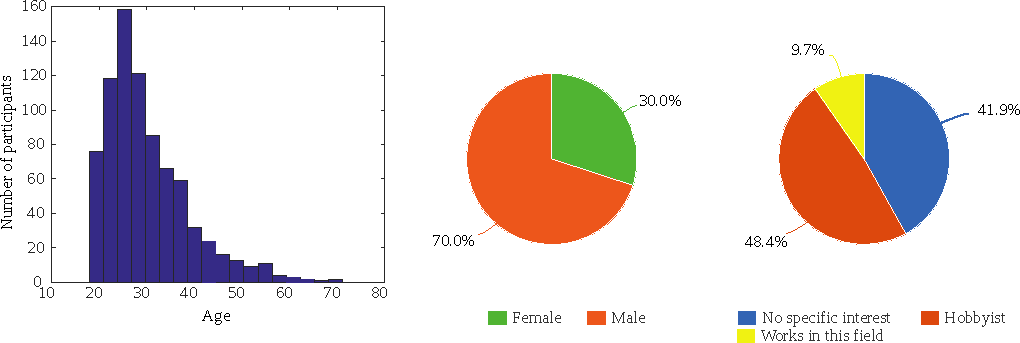
\includegraphics[width=\textwidth]{figures/chapter3/age_gender_cgi.pdf}
\caption{Age, gender, and computer graphics/image processing familiarity distribution of the participants.
%paper
}
\label{fig:age_gender_cgi}
\end{center}
\end{figure}

After collecting the experimental results, it was found that 18747 unique image triplets were judged by the observers. This amounts to approximately 11.6\% of the total possible triplets that can be obtained from 100 images, C(100, 3). Experiment sessions were independent and random for each participant, but it was guaranteed that a single session consisted of only unique triplets. This design resulted in a single response for the majority of the triplets. Some triplets received two responses and only a few received three or more. As such we considered this first phase of the experiment as a random exploration of all possible comparisons. However, as judging similarity based on a single response could be too subjective, we extended the experiment as discussed below to collect multiple responses for each triplet.

The first phase of the experiment was extended to obtain three evaluations per triplet. Unlike the first phase where triplets were generated randomly, the second phase solely used the triplets that had been evaluated before. To achieve this, we sorted the triplets from the first phase in descending order. If a triplet had more than three responses, we randomly selected three of them. Triplets with exactly three responses were used as is. These two cases occurred very rarely. Next, triplets with two responses, and then a single response were presented randomly to obtain a total of 4890 triplets that had been evaluated three times. Among these thrice evaluated triplets, 2172 triplet were judged consistently by all three observers. The remaining 2820 triplets generated two-to-one responses. Similar to the first part of the experiment, the second part also contained the same validity checks to eliminate the responses of inattentive observers.
%paper
\subsection{Phase I}
\subsection{Phase II}








\chapter{Experiment Analysis}
\label{chp:b4}
Having discussed the details of crowdsourcing study in Chapter \ref{chp:b3} and experimented features in Section \ref{sec:features}, this chapter explains how the human judgments and image features are related. First analysis method for assessing the correlation between individual feature type and the experiment results is given. Then, two possible methods to combine the features for developing a more effective similarity model is discussed. In the evaluations, different formats for HDR images are employed in order to measure the effect of the formats of the image format to the proposed methods. 

\section{Preprocessing}
In evaluations, HDR images used directly, as well as by linear scaling and applying several tone mapping operators. For linear scaling, 5\% of the brightest pixels and 5\% of the darkest pixels are discarded by setting them to 95th and 5th percentile of the pixels values respectively. The reason behind this step is to eliminate outlier values from the HDR images that may also introduced by hardware. 

\begin{equation}
    I' = \begin{cases}
    P_5 (I), \text{ if $I < P_5(I)$} \\
    I, \text{ if $P_5(I) \leq I \leq P_{95}(I) $} \\
    P_{95}(I), \text{if $I > P_{95}(I)$}, \\
    \end{cases}
\end{equation}

where $I$ denotes the original image values and $I'$ is after outlier pixel values are removed. Then HDR image is linearly scaled with

\begin{equation}
    lin(I)  = {{I' - I'_{min}} \over {I'_{max} - I'_{min}}}, 
\end{equation}

for each color channel separately.

Besides of using original and linearly scaled HDR images, tone mapped version of the images are also evaluated. For this purpose commonly used tone mapping operators Mai et al. ~\cite{mai2011subjective}, Reinhard et al. (local) ~\cite{reinhard2002photographic}, Reinhard et al. (global) ~\cite{reinhard2002photographic}, Durand \& Dorsey~\cite{durand2002fast}, Mantiuk et al.~\cite{mantiuk2006backward}, Reinhard \& Devlin~\cite{reinhard2005dynamic}, Fattal et al.~\cite{durand2002fast}, Mantiuk et al.~\cite{mantiuk2008modeling}, Ferradans et al.~\cite{ferradans2011analysis} and Pattanaik et al.~\cite{pattanaik2000time} are used. These TMOs are available in opensource PFStmo software library ~\cite{mantiuk2007high}, which provides a reliable implementation of several commonly used TMOs.[!]


\section{Individual Feature Correlation}
%paper
Assume that $t_i = R_i-A_i-B_i$ represents the $i^{th}$ triplet (i.e. trial) with $R_i$ being the reference image, $A_i$ the left test image, and $B_i$ the right test image. This triplet could have been evaluated one or more times by different observers. Let $n(A_i)$ and $n(B_i)$ represent the number of times that each image was found more similar to $R_i$ than the other. From this information, we created a binary vector to encode the participants’ responses:
\begin{equation}
\label{eq:p_vector}
P = (x_1, \ldots, x_N),
\end{equation}

where each element is defined as:
\begin{equation}
x_i = \begin{cases}
1, \text{if $n(A_i) > n(B_i)$}, \\
0, \text{otherwise}.
\end{cases}
\end{equation}

For each feature type $f$, we also computed the feature representations of each image as $f(R_i)$, $f(A_i)$, $f(B_i)$ and computed their similarity to each other to obtain the following binary vector:
\begin{equation}
    F = (y_1,\cdots, y_N ),
\end{equation}
where
\begin{equation}
y_i = \begin{cases}
1, \text{ if $ d(f(R_i), f(A_i)) < d(f(R_i), f(B_i))$ } \\
0, \text{otherwise}.
\end{cases}
\end{equation}

In this equation $d$ represents the distance metric that was chosen to be used for feature $f$. This encoding gave rise to two binary vectors, $P$ and $F$, with the former computed from user responses and the latter from feature similarities. There are many approaches to compute the correlation between two such vectors. We used the Sokal-Michener correlation, which is a simple, intuitive, and effective way to correlate two binary vectors~\cite{zhang2003properties}. This correlation is defined as

\begin{equation}
s = {{S_{11}(P, F) + S_{00}(P, F)} \over {N}},
\end{equation}

with $S_{11}$ and $S_00$ representing the total count of matching ones and zeros respectively:

\begin{equation}
    S_{11}(P, F) = P \cdot F,
\end{equation}
\begin{equation}
    S_{00}(P, F) = \neg P \cdot \neg F, 
\end{equation}


Note that the correlation coefficient s can take a value in range [0, 1]. In the following, we multiply this coefficient by 100 to represent the correlations as percentages.

The raw feature correlations with the first (Section \ref{sec:exp_phase_I}) and the second phase of the experiment (Section \ref{sec:exp_phase_II}) are reported in Tables \ref{tab:ind_correlation_p1} and \ref{tab:ind_correlation_p2}, respectively. In these tables, the leftmost column indicates the processing type applied to the images before the computation of features.

\begin{landscape}
\begin{table}
\caption{Individual feature correlations with the first phase of the experiment. The numbers indicate the Sokal-Michener correlation scaled by 100 to represent percentages.}
\centering
\begin{tabular}{r | c c c c c c c}
\label{tab:ind_correlation_p1}
\textbf{Processing Type} & \textbf{VGG16} & \textbf{VGG19} & \textbf{Color} & \textbf{Luminance} & \textbf{Texture} & \textbf{GIST}\\
\hline
HDR-original & 56.79 & 58.09 & 55.10 & 53.14 & 52.39 & 56.82 \\
HDR-linear & 63.54 & 63.31 & 55.69 & 54.07 & 54.36 & 58.18 \\
Drago et al.~\cite{drago2003adaptive} & 65.88 & 65.74 & 56.73 & 57.45 & 51.17 & 58.23 \\
Mai et al.~\cite{mai2011subjective} & 65.28 & 65.13 & 56.01 & 56.77 & 51.90 & 57.57 \\ 
Reinhard et al. (local)~\cite{reinhard2002photographic} & 65.82 & 65.63 & 56.58 & 54.77 & 51.43 & 57.89 \\
Reinhard et al. (global)~\cite{reinhard2002photographic} & 65.75 & 65.52 & 56.59 & 54.68 & 51.39 & 57.92 \\
Durand \& Dorsey~\cite{durand2002fast} & 66.17 & 65.43 & 55.77 & 55.12 & 51.79 & 57.85 \\
Mantiuk et al.~\cite{mantiuk2006backward} & 65.42 & 65.33 & 56.29 & 55.38 & 52.08 & 58.03 \\
Reinhard \& Devlin~\cite{reinhard2005dynamic} & 65.28 & 65.20 & 57.15 & 55.89 & 54.85 & 58.33 \\
Fattal et al.~\cite{durand2002fast} & 65.90 & 65.72 & 56.39 & 57.46 & 51.92 & 58.19 \\
Mantiuk et al.~\cite{mantiuk2008modeling} & 65.71 & 65.74 & 55.98 & 56.99 & 51.84 & 57.86 \\
Ferradans et al.~\cite{ferradans2011analysis} & 66.02 & 65.90 & 55.18 & 56.51 & 51.99 & 58.33 \\
Pattanaik et al.~\cite{pattanaik2000time} & 64.46 & 64.38 & 53.04 & 54.61 & 53.06 & 57.84 
\end{tabular}
\end{table}
\end{landscape}

\begin{landscape}
\begin{table}
\caption{Individual feature correlations with the second phase of the experiment. The numbers indicate the Sokal-Michener correlation scaled by 100 to represent percentages.}
\centering
\begin{tabular}{r|c c c c c c c}
\label{tab:ind_correlation_p2}
\textbf{Processing Type} & \textbf{VGG16} & \textbf{VGG19} & \textbf{Color} & \textbf{Luminance} & \textbf{Texture} & \textbf{GIST}\\
\hline
HDR-original & 64.88 & 67.14 & 60.23 & 58.39 & 54.42 & 63.50 \\
HDR-linear & 75.58 & 76.13 & 60.78 & 57.79 & 57.97 & 65.71 \\
Drago et al.~\cite{drago2003adaptive} & 80.88 & 81.80 & 62.58 & 62.72 & 53.87 & 65.39 \\
Mai et al.~\cite{mai2011subjective} & 80.00 & 79.95 & 61.11 & 61.66 & 53.46 & 64.06 \\
Reinhard et al. (local)~\cite{reinhard2002photographic} & 80.92 & 81.61 & 62.21 & 58.16 & 53.87 & 64.88 \\
Reinhard et al. (global)~\cite{reinhard2002photographic} & 80.92 & 81.57 & 62.21 & 57.97 & 54.75 & 64.75 \\
Durand \& Dorsey~\cite{durand2002fast} & 81.75 & 81.34 & 62.07 & 59.22 & 53.00 & 64.19 \\
Mantiuk et al.~\cite{mantiuk2006backward} & 80.41 & 80.65 & 61.15 & 59.59 & 52.49 & 64.47 \\ 
Reinhard \& Devlin~\cite{reinhard2005dynamic} & 80.37 & 80.41 & 64.15 & 61.43 & 60.55 & 65.44 \\
Fattal et al.~\cite{durand2002fast} & 80.51 & 80.92 & 62.30 & 64.24 & 52.90 & 65.02 \\
Mantiuk et al.~\cite{mantiuk2008modeling} & 80.00 & 80.78 & 62.12 & 61.71 & 54.56 & 64.19 \\
Ferradans et al.~\cite{ferradans2011analysis} & 81.38 & 82.21 & 58.39 & 61.61 & 55.02 & 65.25 \\
Pattanaik et al.~\cite{pattanaik2000time} & 78.66 & 78.11 & 57.33 & 58.66 & 55.71 & 64.52
\end{tabular}
\end{table}
\end{landscape}

“HDR-original” represents the unaltered HDR image whereas “HDR-linear” represents its linearly scaled version. The other processing types all include the application of a certain tone mapping operator. For all processing types, except the original, the images were gamma-corrected and scaled to [0, 255] range.

\section{Combined Feature Correlation}

Given the individual correlations reported in the previous tables, a natural question that follows is if we can combine them to develop a single objective metric that better correlates with human’s assessment of similarity for HDR images. To this end, we performed two types of linear regression analysis yielding two related but different models.

In both models, closely related deeply learned features VGG16 and VGG19 used as separate features instead of selecting the better performing one. The reason behind this, as the study~\cite{simonyan2014very} suggests, the results obtained from combination of VGG16 and VGG19 (by taking an average) performs better than both VGG16 and VGG19, indicates that VGG16 and VGG19 are complementary features. This claim is consistent with our results given Table \ref{tab:fuse_vgg_phaseI} and \ref{tab:fuse_vgg_phaseII}.

\begin{table}
\caption{Comparison of correlation results for the features VGG16, VGG19 and combination VGG16-19 for the Phase I of the experiment.}
\label{tab:fuse_vgg_phaseI}
\begin{tabular}{r|c|c|c}
\textbf{Processing Type} & \textbf{VGG16} & \textbf{VGG19} & \textbf{VGG16-19} \\
\hline
HDR-original &  56.79 & 58.09 & 57.91 \\
HDR-linear &  63.54 & 63.31 & 63.85 \\
Drago et al.~\cite{drago2003adaptive} &  65.88 & 65.74 & 66.31 \\
Mai et al.~\cite{mai2011subjective} &  65.28 & 65.13 & 66.06 \\
Reinhard et al. (local)~\cite{reinhard2002photographic} & 65.82 & 65.63 & 66.21 \\
Reinhard et al. (global)~\cite{reinhard2002photographic} & 65.75 & 65.52 & 66.29 \\
Durand \& Dorsey~\cite{durand2002fast} & 66.17 & 65.43 & 66.44 \\
Mantiuk et al.~\cite{mantiuk2006backward} & 65.42 & 65.33 & 65.97 \\
Reinhard \& Devlin~\cite{reinhard2005dynamic} & 65.28 & 65.20 & 65.81 \\
Fattal et al.~\cite{durand2002fast} & 65.90 & 65.72 & 66.25 \\
Mantiuk et al.~\cite{mantiuk2008modeling} & 65.71 & 65.74 & 66.01 \\
Ferradans et al.~\cite{ferradans2011analysis} & 66.02 & 65.90 & 66.77 \\
Pattanaik et al.~\cite{pattanaik2000time} & 64.46 & 64.38 & 64.76
\end{tabular}
\end{table}

\begin{table}
\caption{Comparison of correlation results for the features VGG16, VGG19 and combination VGG16-19 for the Phase II of the experiment}
\label{tab:fuse_vgg_phaseII}
\begin{tabular}{c|c|c|c}
\textbf{Processing Type} & \textbf{VGG16} & \textbf{VGG19} & \textbf{VGG16-19} \\
\hline
HDR-original &  64.88  &  67.14  &  66.59 \\
HDR-linear &  75.58   & 76.13 & 76.96 \\
Drago et al. ~\cite{drago2003adaptive} &  80.88 &    81.8 &    82.35 \\
Mai et al. ~\cite{mai2011subjective} &  80 &   79.95    & 81.2 \\
Reinhard et al. (local) ~\cite{reinhard2002photographic} & 80.92 &    81.61 &    82.21 \\
Reinhard et al. (global) ~\cite{reinhard2002photographic} & 80.92   & 81.57   &  82.3 \\
Durand \& Dorsey~\cite{durand2002fast} & 81.75   & 81.34  &  82.76 \\
Mantiuk et al.~\cite{mantiuk2006backward} & 80.41   & 80.65 &   81.24 \\
Reinhard \& Devlin~\cite{reinhard2005dynamic} & 80.37  &  80.41 &    81.24 \\
Fattal et al.~\cite{durand2002fast} & 80.51   & 80.92 &    81.98 \\
Mantiuk et al.~\cite{mantiuk2008modeling} &  80   & 80.78   & 80.51 \\
Ferradans et al.~\cite{ferradans2011analysis} & 81.38 &    82.21 &    83.27 \\
Pattanaik et al.~\cite{pattanaik2000time} & 78.66   & 78.11   & 79.77
\end{tabular}
\end{table}



\subsection{Triplet Model}
%paper
In our first analysis, we aimed to develop a model that
predicts which of the two test images is more similar to the reference image using the pairwise distances between the test and reference images. Assuming that j is a feature index, one can compute these pairwise differences as follows:
\begin{equation}
    a_j = d_j(f_j(R), f_j(A)), 
\end{equation}
\begin{equation}
   b_j = d_j(f_j(R), f_j(B)). 
\end{equation}

Here $d_j$ represents the distance metric chosen for the $j^{th}$ feature. The model takes as input these differences for all features (i.e. $j \in {1, 2, 3, 4, 5, 6}$) and computes their weighted average as its response:

\begin{equation}
    r = c_0 + c_1(a_1 - b_1) + c_2(a_2 - b_2) + c_3(a_3 - b_3)+ c_4(a_4 - b_4) + c_5(a_5 - b_5) + c_6(a_6 - b_6)
\end{equation}
 

To compute the unknown coefficients we used logistic regression as our dependent data (i.e. user responses)
were binary: given one reference and two test images, the user selects either the left image or the right one,
encoded as 1 and 0.

The regression was performed between the two vectors, namely the $P$ vector from Equation \ref{eq:p_vector}, and the model response $R$ comprised of the following elements:
\begin{equation}
    R = (r_1,\cdots, r_N ),
\end{equation}
where
\begin{equation}
    r_i = [a_{i1} - b_{i1} \cdots a_{i6} - b_{i6}].
\end{equation}

The logistic regression models the logarithm of the odds as the response of the model:
\begin{equation}
   ln \left( {{Pr(x = 1)} \over { 1 - Pr(x = 1)}} \right) = r. 
\end{equation}


From this equation, it can be derived that the probability of a user responding 1 (i.e. selecting the left image)
is equal to

\begin{equation}
\label{eq:response_prob}
    Pr(x = 1) = {{1} \over {1 + e^{-r}}}
\end{equation}

If we find $Pr(x = 1) > 0.5$, we assume that the model has selected the left image. Otherwise, the model’s response was taken as the right image.

To measure the effectiveness of this model we used 10-fold cross validation. In each fold, 90\% of the trials
were selected for training and the remaining 10\% for testing. This process was repeated 10 times while ensuring that each test fold is mutually exclusive from each other. Similar to the analysis of individual features, we assessed the success of this model against both the Phase I and the Phase II of the experiment. The results are shown in Table \ref{tab:correlation_triplet_model}. It can be seen that the feature combination, on average, improves the success of each presentation type by about 3\% to 4\%. The best three results are obtained by Ferradans et al.’s~\cite{ferradans2011analysis}, Drago et al.’s ~\cite{drago2003adaptive}, and Reinhard et al.’s ~\cite{reinhard2002photographic} TMO algorithms. The reported coefficients are computed by using the entire dataset from the Phase II of the experiment due to its higher correlation with the combined features.

\begin{landscape}
\begin{table}
\caption{The correlations of the first regression model with the user responses. Phase I and Phase II represent the initial and extended experiments respectively. The coefficients are reported for the Phase II of the experiment only due to its higher correlation with the user data.}
\centering
\begin{tabular}{r|c c || r r r r r r r}
\label{tab:correlation_triplet_model}
\textbf{Processing Type} & \textbf{Phase I} & \textbf{Phase II} & \textbf{c0} & \textbf{c1} & \textbf{c2} & \textbf{c3} & 
\textbf{c4} & \textbf{c5} & \textbf{c6}\\
\hline
HDR-original & 60.67 & 70.76 & 0.0573 & 0.0768 & -3.3241 & -0.0028 & -0.0124 & -0.2921 & -10.7505 \\
HDR-linear & 64.81 & 78.83 & 0.0005 & -5.4801 & -5.9902 & -0.0074 & -0.0635 & -0.3289 & -10.1782 \\
Drago et al. ~\cite{drago2003adaptive} & 67.36 & 83.49 & -0.0423 & -7.8751 & -7.6339 & -0.0506 & -0.0958 & 0.0043 & -7.3615 \\
Mai et al. ~\cite{mai2011subjective} & 66.70 & 81.78 & 0.0085 & -5.2932 & -7.9526 & -0.0601 & -0.1078 & -0.0358 & -4.9275 \\
Reinhard et al. (local) ~\cite{reinhard2002photographic} & 67.19 & 83.21 & -0.0154 & -7.3838 & -8.7207 & -0.0688 & -0.0853 & 0.0145 & -7.8380 \\
Reinhard et al. (global) ~\cite{reinhard2002photographic} & 67.34 & 83.16 & -0.0230 & -7.0932 & -8.8856 & -0.0687 & -0.0783 & 0.0101 & -7.4470 \\
Durand \& Dorsey~\cite{durand2002fast} & 66.92 & 83.03 & -0.0604 & -8.1694 & -7.3044 & -0.0977 & -0.0147 & 0.0082 & -6.8549 \\
Mantiuk et al.~\cite{mantiuk2006backward} & 66.64 & 81.74 & 0.0220 & -6.1999 & -8.0462 & -0.1081 & -0.0286 & -0.0102 & -10.0494 \\
Reinhard \& Devlin~\cite{reinhard2005dynamic} & 66.72 & 82.75 & -0.0332 & -5.6555 & -8.8871 & -0.1284 & -0.0144 & -0.0254 & -7.9970 \\
Fattal et al.~\cite{durand2002fast} & 67.25 & 82.56 & -0.0025 & -6.2320 & -8.3176 & -0.1120 & -0.0272 & -0.0143 & -7.9175 \\
Mantiuk et al.~\cite{mantiuk2008modeling} & 66.91 & 82.15 & -0.0005 & -5.7555 & -8.4433 & -0.0777 & -0.0548 & -0.0041 & -6.8189 \\
Ferradans et al.~\cite{ferradans2011analysis} & 67.21 & 83.53 & 0.0226 & -5.7782 & -9.8899 & -0.0801 & -0.0432 & -0.0060 & -7.4090 \\
Pattanaik et al.~\cite{pattanaik2000time} & 65.02 & 79.89 & -0.0365 & -7.5194 & -5.6052 & 0.0132 & -0.0565 & 0.0211 & -6.1389 \\
\end{tabular}
\end{table}
\end{landscape}


%paper
\subsection{Duplet Model}
Despite the first regression model yielding high correlations exceeding 80\% for most algorithms, it has an important drawback. It requires a triplet of images, one reference and two test, as input to the model. While this matches the presentation type in our experiment, a more desirable model should be able to take only two images (e.g., a query image and a test image) and produce a relative similarity score between them. This may allow, for instance, ranking the similarity of multiple images with a query image as in image-based search applications.

In order to allow for this possibility, our second regression model was designed in the following manner.
For each trial, $ti = R_i - A_i - B_i, i \in {1, \cdots , N}$, we inserted two elements to our user response vector:
\begin{equation}
    x_{2i-1} = \begin{cases} 
    1, \text{ if $n(A_i) > n(Bi)$ } \\
    0, \text{otherwise},
    \end{cases}
\end{equation}
\begin{equation}
    x_{2i} = \neg  x_{2i-1},
\end{equation}
    

yielding a vector of size $2N$:
\begin{equation}
   P = (x_1, x_2,\cdots, x_{2N} ). 
\end{equation}

As for the model’s inputs each element of the feature vector was computed as
\begin{equation}
    y_{2i-1} = [a_1 \cdots a_6], 
\end{equation}
\begin{equation}
    y_{2i} = [b_1 \cdots b_6], 
\end{equation}


yielding
\begin{equation}
    F = (y_1, y_2, \cdots , y_{2N} ).
\end{equation}

In summary, the elements of the feature vector always followed the A, B order, whereas the corresponding elements in the user vector were 1 for the selected image and 0 for the other image. This second regression model learns to produce the following response given the feature differences between a reference and test image:

\begin{equation}
\label{eq:log_regression}
    r_a = c_0 + c_1a_1 + c_2a_2 + c_3a_3 + c_4a_4 + c_5a_5 + c_6a_6 
\end{equation}

By converting this response to probability values as in Equation \ref{eq:response_prob}, one can compute a relative degree of similarity between the two images. To validate this model, we computed the model response twice by using $R_i - A_i$ and $R_i - B_i$ image pairs:
\begin{equation}
    Pr(x = left) = {{1} \over {1 + e^{-r_a}}} 
\end{equation}
\begin{equation}
    Pr(x = right) = {{1} \over {1 + e^{-r_b}}}
\end{equation}


Given a triplet, if we found $Pr(x = left) > Pr(x =right)$ we assumed the model to have selected the left image. Otherwise, it was assumed that the model selects the right one. The correlation of this model with the user responses was calculated as in the previous model yielding the results in Table \ref{tab:correlation_duplet_model}. The best result of the second model was found for Drago et al.’s ~\cite{drago2003adaptive} TMO in the extended experiment. The model achieved a correlation of 83.81\% with the user responses. Similarly to the Triplet Model, the reported coefficients are computed by using the entire dataset from the Phase II of the experiment due to its higher correlation with the combined features.

\begin{sidewaystable}
\caption{The correlations of the second regression model with the user responses. Phase I and Phase II represent the initial and extended experiments respectively. The coefficients are reported for the Phase II of the experiment only due to its higher correlation with the user data.}
\centering
\begin{tabular}{r|c c || r r r r r r r}
\label{tab:correlation_duplet_model}
\textbf{Processing Type} & \textbf{Phase I} & \textbf{Phase II} & \textbf{c0} & \textbf{c1} & \textbf{c2} & \textbf{c3} & 
\textbf{c4} & \textbf{c5} & \textbf{c6}\\
\hline
HDR-original & 60.75 & 70.80 & 2.9323 & -0.1531 & -2.8191 & -0.0024 & -0.0063 & -0.2494 & -7.1569 \\
HDR-linear & 64.65 & 78.50 & 5.5623 & -3.9224 & -3.7111 & -0.0149 & -0.0048 & -0.2164 & -5.5490 \\
Drago et al. ~\cite{drago2003adaptive} & 67.52 & 83.81 & 8.3967 & -5.5248 & -4.0845 & -0.0280 & -0.0587 & -0.0054 & -3.3575 \\
Mai et al. ~\cite{mai2011subjective} & 66.72 & 81.73 & 7.4594 & -4.0822 & -5.0859 & -0.0196 & -0.0532 & -0.0326 & -0.9064 \\
Reinhard et al. (local) ~\cite{reinhard2002photographic} & 67.35 & 83.53 & 8.2123 & -5.6104 & -4.3743 & -0.0249 & -0.0290 & 0.0063 & -3.6705 \\
Reinhard et al. (global) ~\cite{reinhard2002photographic} & 67.20 & 83.16 & 8.2162 & -5.3915 & -4.5828 & -0.0259 & -0.0264 & 0.0049 & -3.6673 \\
Durand \& Dorsey~\cite{durand2002fast} & 66.81 & 82.61 & 8.2396 & -5.9298 & -4.0539 & -0.0560 & -0.0081 & 0.0077 & -3.1001 \\
Mantiuk et al.~\cite{mantiuk2006backward} & 66.50 & 82.10 & 7.6833 & -4.3626 & -4.8232 & -0.0658 & -0.0212 & -0.0082 & -3.4889 \\
Reinhard \& Devlin~\cite{reinhard2005dynamic} & 66.56 & 82.61 & 8.5676 & -4.6656 & -4.9324 & -0.0936 & -0.0075 & -0.0262 & -2.8843 \\
Fattal et al.~\cite{durand2002fast} & 67.07 & 82.79 & 8.0671 & -4.4119 & -4.8215 & -0.0716 & -0.0191 & -0.0141 & -2.8938 \\
Mantiuk et al.~\cite{mantiuk2008modeling} & 66.57 & 82.01 & 7.7805 & -3.9872 & -5.3899 & -0.0228 & -0.0319 & -0.0084 & -2.6625 \\
Ferradans et al.~\cite{ferradans2011analysis} & 67.33 & 83.16 & 8.5911 & -5.0432 & -4.9965 & -0.0541 & -0.0258 & -0.0089 & -2.3825 \\
Pattanaik et al.~\cite{pattanaik2000time} & 64.94 & 79.84 & 6.6735 & -5.6657 & -3.4601 & 0.0109 & -0.0295 & 0.0241 & -1.8922
\end{tabular}
\end{sidewaystable}

\chapter{Application: Style Based Tonemapping}
\label{chp:b5}

\section{Problem Definition}

Tone mapping operators aim to reduce the dynamic range of an HDR image to display it on an low dynamic range display devices. The existence of numerous tone mapping operators that are available paved the way for many studies that are conducted for selecting the best one~\cite{parraga2018tone}. However, tone mapping can be conducted for different purposes, and rendering the resulting images to follow a consistent style can be one of them. For example, in a movie production process, making all frames consistently tone mapped, regardless of the content of the frames, can be a desired operation to impart a certain look and feel to the viewers. Although obtaining different renderings from tone mapping operators is partly achievable by using different tone mapping parameters, some tone mapping operators have none~\cite{Dura02} or few parameters~\cite{Fatt02} while others~\cite{Photomatix2010} have too many. Besides, even though one set of parameters are found for a certain image to depict a certain style of rendering, the same set of parameters would not yield with the same look when applied to other images. %that has different characteristics.

In this chapter, we propose a style based tone mapping operator that aims to consistently tone map different HDR images with the defined style.Figure \ref{fig:styles} shows different styles for the same images created by an artist. In this study, we approach the problem of defining a style by presenting the user an HDR image and with the help of the tool developed, ask the user to change the parameters until the image matches the desired look. By repeating this process for a small set of calibration images, we aim to \emph{learn} the style. Applying the learned style from calibration images to the previously unseen images is essentially a visual image similarity problem.

\begin{figure}
\begin{center}
\includegraphics[width=\textwidth]{figures/chapter5/styles.png}
\caption{Different artists may prefer different tone reproductions of the same HDR image. The same artist may also choose to produce different styles based on the situational/contextual considerations. The images reproduced by a professional artist using a different tool (top half) are replicated using our operator (bottom half). Our algorithm can also learn the styles of an artist and produce results consistent with them.}
\label{fig:styles}
\end{center}
\end{figure}

First, the problem of relating the input HDR image and the calibration images are solved with a method that has been commonly used for LDR images in the earlier work and then we employ two different but related methods that uses the findings from the user experiment of visual similarity for HDR images discussed in Chapter \ref{chp:b3} and Chapter \ref{chp:b4}. 


\section{Related Work}
Image reproduction is ultimately a subjective process where photographers and artists of all persuasions are free to reflect their own interpretation into the final rendering. For any task of reproduction, there is generally a vast range of choices from literal or realistic reproduction to those that significantly depart from reality. Since the early days of photography, many tools and systems have been developed to enable artists express their creativity~\cite{Adams80,Adams81,Adams83,White84}.

Tone mapping, in the context of HDR imaging, is no different in creative expression than the art of photography. There is essentially an infinite amount of choices that an artist can make when tone mapping an HDR image for display purposes (Figure~\ref{fig:styles}). Perhaps, this is underscored by the large number of TMOs that have so far been developed that produce different outputs from the same HDR image~\cite{Rein2010}.

However, most TMOs fail to provide sufficient freedom to artists to express their creativity. Some operators have specific goals such as preserving brightness~\cite{Tumb93}, contrast~\cite{Duan2004}, visibility~\cite{Ward97,yang2018adaptive}, and photographic look~\cite{Rein2002a}. Others, model the human visual system (HVS) to mimic the perceptual response of a human observer~\cite{Ferw96,Patt98,Meylan2006,khan2017tone}, sometimes also accounting for color appearance~\cite{Kuang2007,Reinhard2012} and device characteristics~\cite{Mantiuk2008}. Yet other operators provide parameter-free or a few parametered solutions that do not model the visual mechanisms but nevertheless produce good results~\cite{Dura02,Fatt02}.

On the contrary, there are a few TMOs that are designed to enable artistic freedom such as the stroke-based interface that was proposed by Lischinski et al.~\cite{Lischinski2006}. This algorithm allows the user to select image regions using brush strokes and set different tone mapping parameters for each region. These parameters are then extrapolated to the entire image using an edge-preserving energy minimization method. Paris et al.~\cite{paris2011local} gives users the possibility of enhancing details or edge-preserving smoothing while tone mapping. This method first applies detail modifying local Laplacian filters on the log intensity of the image and then map the intensities to displayable range by scaling.  

Another algorithm that allows a wide range of possibilities during tone mapping is the generic TMO~\cite{Mantiuk08a}. This operator hinges on the idea that although a large number of TMOs exist, the majority of them can be modeled using a generic tone curve followed by local modifications. The authors have demonstrated that by using a small set of parameters, a skilled artist can match the output of any TMO with the generic TMO. Although these algorithms offer expressive freedom to the artist, they have no notion of \emph{learning} the artist's preference. In fact, it has been shown by the authors that the same set of parameters can give rise to vastly different outputs for different images~\cite{Mantiuk08a}. As such, using these operators to automatically tone map a large number of images is impractical. 

Of most similar to our work are the LDR retouching studies that allow enhancing a new image using a set of previous training examples~\cite{kang2010personalization, bychkovsky2011learning} or by automatic exposure correction~\cite{yuan2012automatic} or artistic enhancement~\cite{son2014art}. However, their focus is not HDR image tone mapping.

Recently, deep neural networks are also used for learning image adjustment parameters. Some of these studies uses a training set of high quality images and learns the enhancement parameters in an unsupervised manner~\cite{park2018distort, chen2018deep,ignatov2018wespe}. These methods aim to enhance the general quality of the given image instead of applying a specific style. Yan et al.~\cite{yan2016automatic} on the other hand, proposes to learn a computation model of a style from image pairs, an untouched image and a stylized version. Their method incorporates high level semantic information of the pixels as well as local and global features of the image. Another study with a similar goal, HU et al.~\cite{hu2018exposure} uses unpaired data, a set of stylized images, for learning an operation sequence that will style an input image when applied. The benefit of learning modification steps is it makes the style explainable, which most of the deep learning based image enhancements methods lack. Similar to the previous LDR retouching studies, these methods also do not aim to tone map HDR images.

To summarize, the primary difference of the current method from the earlier work is its ability to learn about the various tone mapping styles that may be desired by an artist from a small set of calibration images. These styles can then be applied when tone mapping a new HDR image. Our algorithm is the first of its kind that gives the ability to batch process a large number of HDR images with respect to different styles.

\section{Method}
Style based tone mapping ~\cite{akyuz2013style} consists of two consecutive phases, namely \emph{calibration} and \emph{operation}. Calibration is the phase where the user defines a style and operation is the phase that the user given HDR image is tone mapped with the predefined style in the calibration phase. Figure \ref{fig:calibration_operation} shows the style based tone mapping algorithm steps and these steps are explained in detail in the following sections.

\begin{figure}
\begin{center}
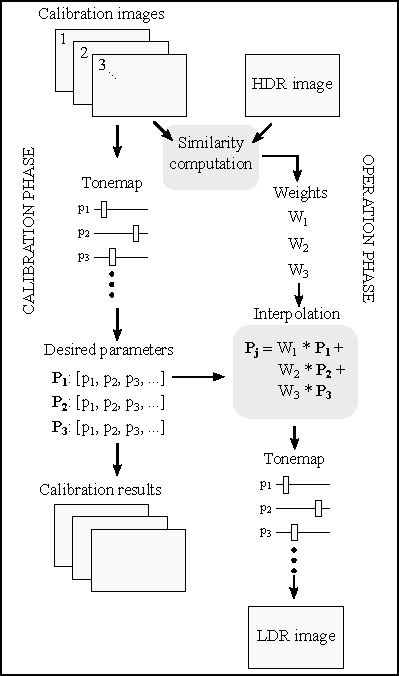
\includegraphics[width=0.6\textwidth]{figures/chapter5/algorithm.pdf}
\caption{Style based tone mapping is comprised of a calibration and operation phase. The artist tone maps several images during calibration which results in a set of parameters. During operation, these parameters are interpolated based on image similarity to find the tone mapping parameters for the given image.}
\label{fig:calibration_operation}
\end{center}
\end{figure}

\subsection{Calibration}
In the calibration phase, first the user is asked to pick a name for the new style to be created, and then the user is required to tone map a fixed set of calibration images. Assigning a name to the style would be helpful for the user to stay consistent with the style while tone mapping the calibration images and once the style is created and saved, will be helpful to have many predefined styles in preset library and reuse them. 

Calibration images should be representative enough for different environments that has different characteristics and distinctive from each other to keep the number of the calibration images low. The number of calibration images directly affects the duration of the calibration phase, so although more calibration images would represent different environments better, in order not to overwhelm the user, the number of calibration images is chosen in a way that the user can finish the calibration phase in a reasonable time.

Calibration images are selected in a semi automatic way. First, all images are taken from Fairchild's HDR image dataset~\cite{fairchild2007hdr} and then converted a feature space and using k-means algorithm divided into different clusters. After clusters are obtained, one calibration image is hand-selected from each cluster, yielding 6 calibration images in total, which are shown in Figure \ref{fig:calibration_images}.

\begin{figure}
\begin{center}
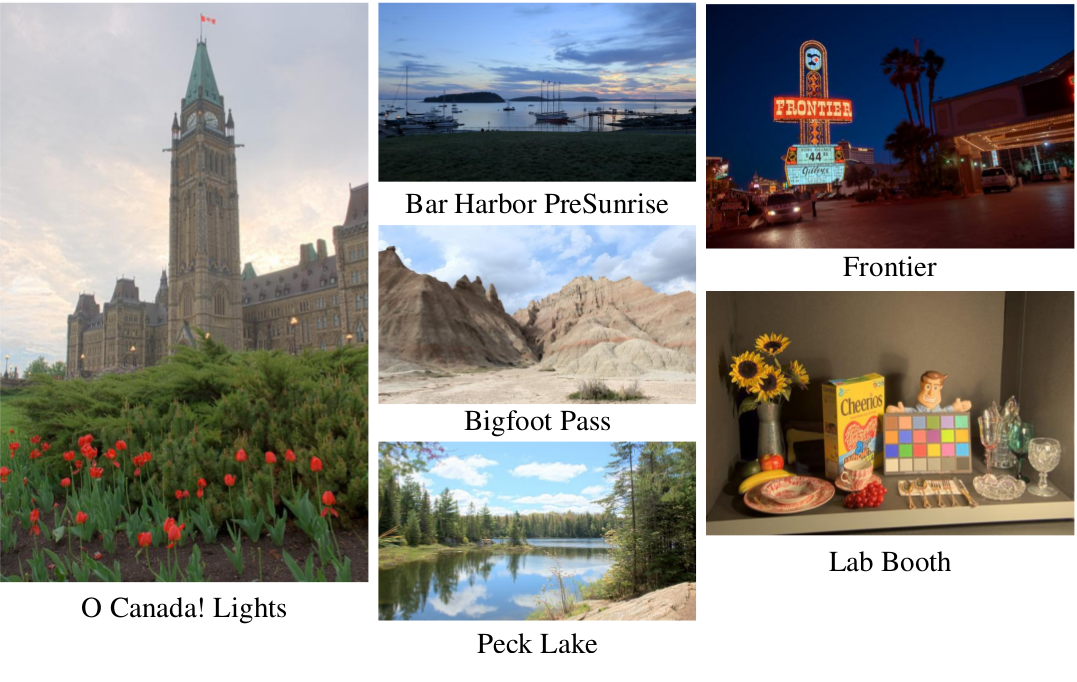
\includegraphics[width=\textwidth]{figures/chapter5/temp_calibration_images.png}
\caption{Calibration images
%paper
}
\label{fig:calibration_images}
\end{center}
\end{figure}

After naming the style, the user is presented with the tone mapping interface and required to tone map the calibration images one after another with the desired style. The manual tone mapping procedure is basically adjusting tone mapping parameters given in Table \ref{tab:tonemap_parameters}.

\begin{table}[h!]
\caption{Tone mapping parameters for style-based tone mapping}
\label{tab:tonemap_parameters}
\centering
\begin{tabular}{|c|c|}
\hline 
Brightness ($b$) & Prct. mapped to half-max intensity \\
Contrast ($c$) & Slope of the tone curve at $b$ \\
Black point ($bp$) & Prct. clamped to min intensity \\
White point ($wp$) & Prct. clamped to max intensity \\
Color saturation ($c$) & Saturation control exponent \\
\hline
Small detail strength ($\lambda_s$) & UM factor for small details \\
Medium detail strength ($\lambda_m$) & UM factor for medium details \\
Large detail strength ($\lambda_l$) & UM factor for large details \\
\hline
\end{tabular}
\end{table}

The tone mapping operator is a modified version of Generic TMO~\cite{mantiuk2008modeling}. Generic TMO models many existing tone mapping operator, both local and global with a tone curve followed by a spatial modulation function. It is note in~\cite{mantiuk2008modeling} that same set of parameters yields very different results for different images. Style based tone mapping uses Generic TMO with the following modifications.

Tone mapping parameters of Generic TMO are replaced with their percentile counterparts in order to make the algorithm less image dependent. For example, the parameter \emph{Brightness} in style based tone mapping with the value 50 would correspond to the median brightness value of the HDR image in Generic TMO's \emph{b} parameter. Likewise, for the parameter \emph{White point}, the value 95 would mean 5\% of the brightest pixels will be burned out. As one may imagine, representing the tone mapping parameters as percentiles is not sufficient to achieve the same effect on different images. In order to achieve this, style based tone mapping uses parameter interpolation to use \emph{similar} parameters to \emph{similar} images as described in Section \ref{sec:operation}. 

The second modification to Generic TMO belongs to spatial modulation. In ~\cite{mantiuk2008modeling}, a linear combination of band-pass filters as spatial modulation function. These filters are from modified Cortex transform and applied after global tone curve modulation. On the other hand, in style based tone mapping, local modulation is applied in multiple scales and then global operation is performed. This has the benefit of adjusting detail level before the HDR compression and gives better results. 

For detail modulation several approaches has been tested, unsharp masking (UM), bileteral filtering~\cite{Tomasi98} and gradient reversal removed BF~\cite{Bae2006}. While BF-based filters results with less halo, they are computationally expensive, unlike UM, which is prone to halos but computationally efficient. Besides, UM is shown to be improve sharpness and local contrast in an earlier study~\cite{Trenta2012}. It is decided to use UM even though it may introduce halos. For some cases, halos may be also introduced by the user in order to create an unrealistic style.

The detail modulation is achieved by first creating three low-pass images in the logarithmic domain for $small$, $medium$ and $large$ details.

\begin{align}
L'_{\sigma_s} = g _{\sigma_s} * L', \\
L'_{\sigma_m} = g _{\sigma_m} * L', \\
L'_{\sigma_l} = g _{\sigma_l} * L', 
\end{align}

where $L' = log L$ and $g_\sigma$ are 2D Gaussian filters are different scales. $\sigma_s$, $\sigma_m$, and $\sigma_l$ are set to 0.0625\%, 0.3125\% and 0.625\% of the minimum image dimension respectively. Then these low pass images are used to enhance different scales with the chosen detail factor parameters $\lambda$.

\begin{equation}
    L_{sm} = e^{L' + \lambda_s(L' - L'_{\sigma_s}) + \lambda_m(L'_{\sigma_s} - L'_{\sigma_m}) + \lambda_l(L'_{\sigma_m} - L'_{\sigma_l})}
\end{equation}

$L_{sm}$, spatially modulated luminance image, then fitted to the tone curve as in~\cite{mantiuk2008modeling}. 

\begin{equation}
    TC(L_{sm}) = 
    \begin{cases}
    0 \text{  if  $L_{sm}' \leq b - d_l$ } \\
    \frac{1}{2}c {{L_{sm}' - b}\over{1 - a_l(L_{sm}'-b)}} + \frac{1}{2} \text{ if $b - d_l < L_{sm}' \leq b $ } \\ 
    \frac{1}{2}c {{L_{sm}' - b}\over{1 + a_h(L_{sm}'-b)}} + \frac{1}{2} \text{ if $b < L_{sm}' \geq b + d_h$} \\ 
    1 \text{ if  $L_{sm}' > b + d_h$}
    \end{cases}
\end{equation}

where $L_{sm}'$ is the logarithm of the spatially modulated luminance $c$ is the contrast, and parameters $b$, $d_l$ and $d_h$ are the absolute values of the user given parameters in percentiles for brightness, black point and white point respectively. Parameters $a_h$ and $a_l$ are contrast compression for light and dark areas computed from ~\cite{mantiuk2008modeling}.

\begin{equation}
    a_l = {{c . d_l-1} \over {d_l}} \text{ and } a_h = {{c . d_h-1} \over {d_h}}
\end{equation}

In Figure \ref{fig:calibration_phase}, the user interface that allows the user to define a style for tone mapping during the calibration phase is shown. The tone mapping parameters can be easily adjusted with the sliders and the calibration image will be tone mapped and shown to the user in real time. The luminance histograms of log HDR and LDR images are also shown to aid the user and show the effect of the changes. After all of the calibration images are tone mapped, the style parameters are saved and the calibration phase finishes.

\begin{sidewaysfigure}
\begin{center}
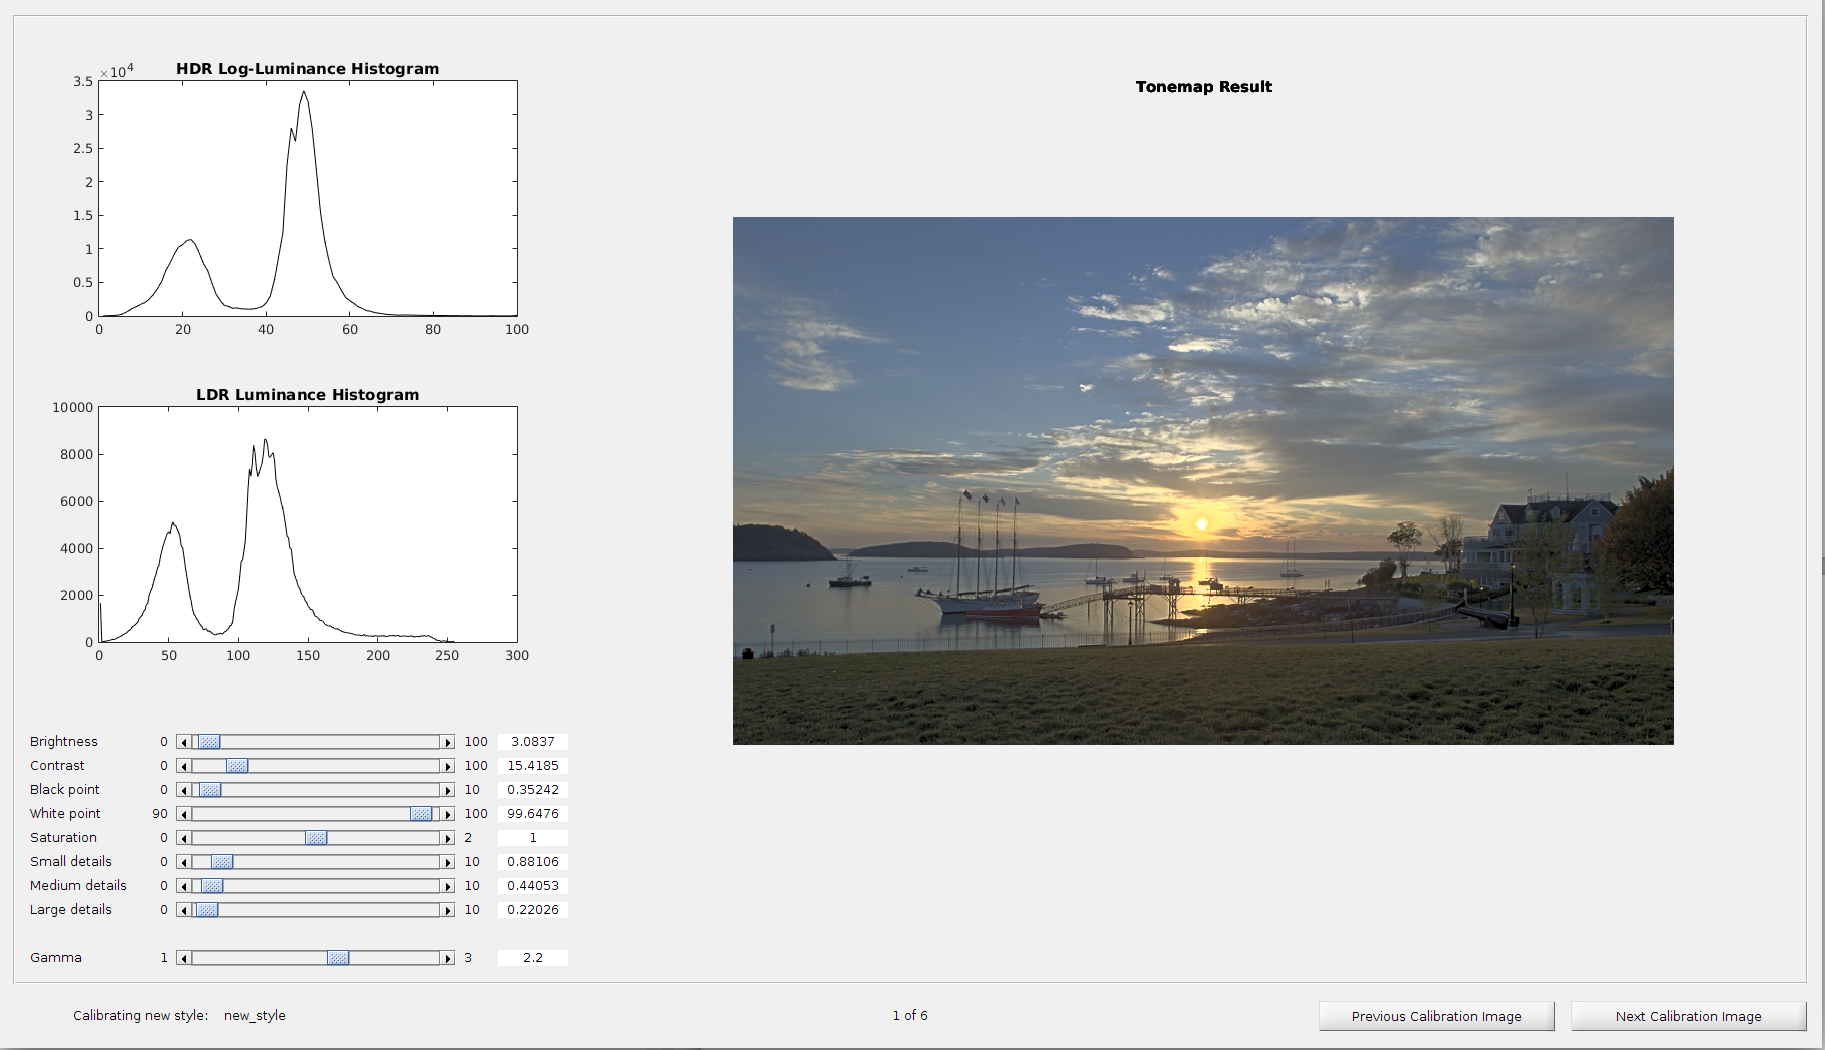
\includegraphics[width=\textwidth]{figures/chapter5/ui_screenshot.png}
\caption{User interface for calibration phase}
\label{fig:calibration_phase}
\end{center}
\end{sidewaysfigure}

\subsection{Operation}
\label{sec:operation}
In the operation phase, user selects a style from preset library that has been created in the calibration phase. Given a new HDR image to be tone mapped with the selected style, the tone mapping parameters \emph{t} (given in Table \ref{tab:tonemap_parameters}) must be determined based on calibration image tone mapping parameters \emph{$t_i$}. Style based tone mapping approaches this problem as image similarity problem. If two images are similar according to a similarity metric, their tone mapping parameters should be also similar. After the distances between input image and the calibration images, the tone mapping parameters are calculated as inverse distance transform~\cite{Shepard1968}:

\begin{equation}
\label{eq:inv_distance_transform}
    \mathbf{t} = {{\sum _{i=1} ^{N} {1 \over {d(\mathbf{f}, \mathbf{f_i})}} \mathbf{t_i}} \over {\sum _{i=1} ^{N} {1 \over {d(\mathbf{f}, \mathbf{f_i})}}}}
\end{equation}

Here, $\mathbf{f}$ is the feature vector of the current input image and $\mathbf{f_i}$ the feature vector for the calibration image $i$ and $\mathbf{t}$ its computed tone mapping parameters. Lastly, the function $d$ calculates the similarity between two feature vectors.

In~\cite{akyuz2013style}, images are represented with HSV histograms~\cite{Ben2006} and histograms of gradients~\cite{dalal2005histograms} to capture colorimetric and structural properties of the images. HDR images varies highly on pixel values and it is hard to compare them directly. To overcome this, images are tone mapped to the interval $[0,1]$:

\begin{equation}
    L_{out} = {{L_{in}} \over {1 + L_{in}}}, 
\end{equation}

and color channels are transformed with:

\begin{equation}
    \mathbf{C_{out}} = {{\mathbf{C_{in}}}\over{L_{in}}} L_{out}.
\end{equation}

The feature vector is then computed using transformed values, as a $60$ dimensional vector, $3x15$ bins for HSV histogram and $15$ bins for gradient histogram. 

Unfortunately, treating histograms as high dimensional points and computing their Euclidean distances does not yield correct results as this ignores the proximity information of the bins. For instance, although the histogram $H1 = (1, 0, 0, \cdots, 0)$ is closer to
$H2 = (0, 1, 0, \cdots, 0)$ than $H3 = (0, 0, 1, \cdots, 0)$, their Euclidean distances are equal. To circumvent this problem, we convolved each histogram with a 1-D Gaussian $(\sigma = 0.7)$ prior to computing their distances ~\cite{Ben2006}. Circular similarity of the hue histogram is also accounted. Thus the final distance metric between two feature vectors \textbf{$f_i$} and \textbf{$f_j$} become:

\begin{equation}
    d(\mathbf{f_i, f_j}) = \mathbf{(f_i - f_j)}^T\mathbf{(f_i-f_j)},
\end{equation}

where \textbf{$f$} is the combined histogram. This metric is used to measure the similarity between input HDR image and calibration images. Also the same distance metric is used to cluster Fairchild dataset in order to pick calibration images.

After tone mapping parameters are calculated with parameter interpolation, HDR image is tonemapped and presented to the user in a similar user interface like Figure \ref{fig:calibration_images}. User can do the final adjustments and save the tone mapped LDR image. Figure \ref{fig:gallery} shows a gallery of our results. Note that despite the large variation of the image content, the selected styles are successfully applied to each image.

\begin{figure}
\begin{center}
\includegraphics[width=\textwidth]{figures/chapter5/gallery.png}
\caption{All of these images are automatically tone mapped using the four styles that are generated.}
\label{fig:gallery}
\end{center}
\end{figure}

\section{Improvements with User Study Results}
Although style based tone mapping has achieved some success for consistently tone mapping different images, the image similarity method given in Section \ref{sec:operation} can be improved with the findings from the conducted user study. In this section, two modifications of this method that are made possible by the experimental findings of the user study is given.

\subsection{Parameter Interpolation with All Features}

In the first modification, features given in Table \ref{tab:table_feature} are extracted from the selected HDR image and calibration images. Then, distances between these features are calculated separately using the corresponding distance metrics given in the same table. The weighted average of these feature distances are calculated using the coefficients obtained from the logistic regression model (Equation \ref{eq:log_regression}), with the idea that less important features should also contribute less to the distance. This operation can be summarized with the following equation:
\begin{equation}
    d_i = \sum_{j=1}^{6}c_j d_j(\mathbf{f_i}, \mathbf{f_{ij}})
\end{equation}

where $c_j$ is the coefficient of the $j^{th}$ feature, $\mathbf{f_j}$ is the $j^{th}$ feature of the input image, $\mathbf{f_{ij}}$ is the same for the $i^{th}$ calibration image, and finally $d_j$ is the distance metric for the $j^{th}$ feature. The result $d_i$ represents the combined distance between the input image and the corresponding calibration image. These combined distances are calculated between the selected HDR image and all calibration images. The tone mapping parameters for the selected HDR image are then interpolated using inverse distance transform as in Equation \ref{eq:inv_distance_transform}. This method differs from the original one in several aspects: 

\begin{itemize}
    \item Using a different and more representative set of features, luminance which is one of the most important features of HDR images has a separate feature vector,
    \item More suitable distance metrics for feature types, for example, EMD takes into account bin proximity for calculating differences between histograms,
    \item Instead of using a single fused feature vector, each feature distance calculated separately,
    \item Employing a weighted average of feature vector distances with weights obtained from a user experiment, compared to using equal weight.
\end{itemize}


\subsection{Parameter Interpolation with Related Features}
While the previous approach calculates a single distance value between images and use this value to interpolate all tone mapping parameters, the second modification relates model features with tone mapping parameters and interpolates individual tone mapping parameters with different weights. To achieve this, we use the relationships defined in Table \ref{tab:feature_mapping}.

\begin{table}
\caption{Model features used for interpolation of tone mapping parameters used in Version II.}
\centering
\begin{tabular}{l | l}
\label{tab:feature_mapping}
\textbf{Tone mapping parameter} & \textbf{Model feature}\\
\hline
Brightness ($t_b$) & Luminance \\
Contrast ($t_c$) & Luminance \\
Black point ($t_{bp}$) & Luminance \\
White point ($t_{wp}$) & Luminance \\
Color saturation ($t_s$) & Color \\
Small detail strength ($t_{\lambda_s}$) & Texture \\
Medium detail strength ($t_{\lambda_m}$ ) & Texture \\
Large detail strength ($t_{\lambda_l}$) & Texture
\end{tabular}
\end{table}


For example, the brightness parameter $t_b$  is computed by interpolating the $t_{b_i}$ parameters of the calibration images by using the similarity of the luminance features:
\begin{equation}
   t_b = { {\sum_{i=1}^N { {1} \over {d_{lum} (lum, lum_i)} } t_{b_i} } \over {\sum_{i=1}^N} { {1} \over {d_{lum} (lum, lum_i)} } }
\end{equation}

Other parameters are interpolated analogously. Because GIST and deep learning features are not directly linked to a specific appearance phenomenon but are measures of overall similarity, we did not directly link them to specific tone mapping parameters. Instead we experimented with merging them using the individually interpolated parameters as follows:
\begin{equation}
   \mathbf{t} = w_0\mathbf{t_0} + w_1\mathbf{t_1} + w_2\mathbf{t_2}, 
\end{equation}

where $\mathbf{t_0}$ represents individually interpolated TMO parameters, $\mathbf{t_1}$ TMO parameters interpolated as a whole using GIST similarity only, and $\mathbf{t_2}$ TMO parameters interpolated as a whole using solely deep learning feature similarity. The weights control the influence of TMO parameters that are computed by using these different approaches.

\section{Results}
In Figure~\ref{FigStyle}, we compare several results obtained by using the original style based tone mapping method as well as with the modifications proposed above. In the first row, we show the results of
the ``Paul Bunyan'' scene from the HDR Photographic Survey~\cite{fairchild2007hdr}. This scene depicts a bright outdoors environment with colorful foreground objects. It may be noted that all results are similar but the individual parameter interpolation with equally weighted GIST and deep learning features (d) has slightly higher contrast (please refer to supplementary full resolution images for better comparison). The overall colorful style is preserved in all images. In the second row, we show the ``Peppermill'' night scene from the same dataset. For this scene the difference of Version II is more clear as images in (c) and (d) exhibit a darker rendering, which is more suitable for a night scene. The reason for this darkening effect is that the $t_b$ parameter for tone mapping becomes more similar to the $t_b$ parameter of the night image in the calibration set due to the similarity of the \emph{luminance} features between these images. The addition of GIST and deep learning features in (d) yields a slightly brighter image compared to (c). We encourage the readers to refer to the electronic supplementary materials for more clear observation of the differences.

\begin{landscape}
\begin{figure}
\begin{subfigure}[b]{0.40\textwidth}
    \centering
    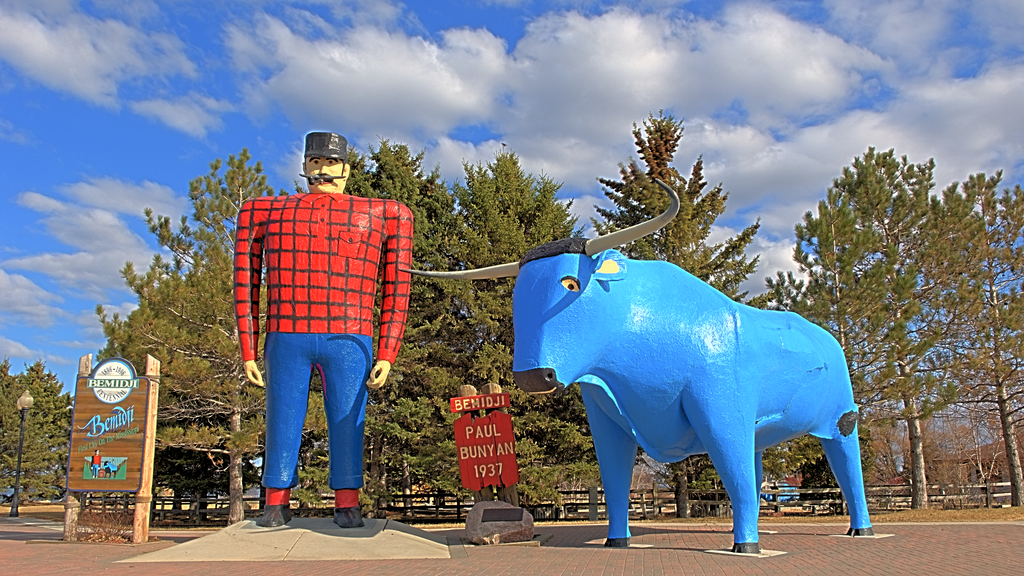
\includegraphics[width=\textwidth]{figures/chapter5/style_based/PaulBunyan_hdrcandy_v1.png}
    \caption{Original}
    \label{FigStyle:original}
\end{subfigure}\hfill
\begin{subfigure}[b]{0.40\textwidth}
    \centering
    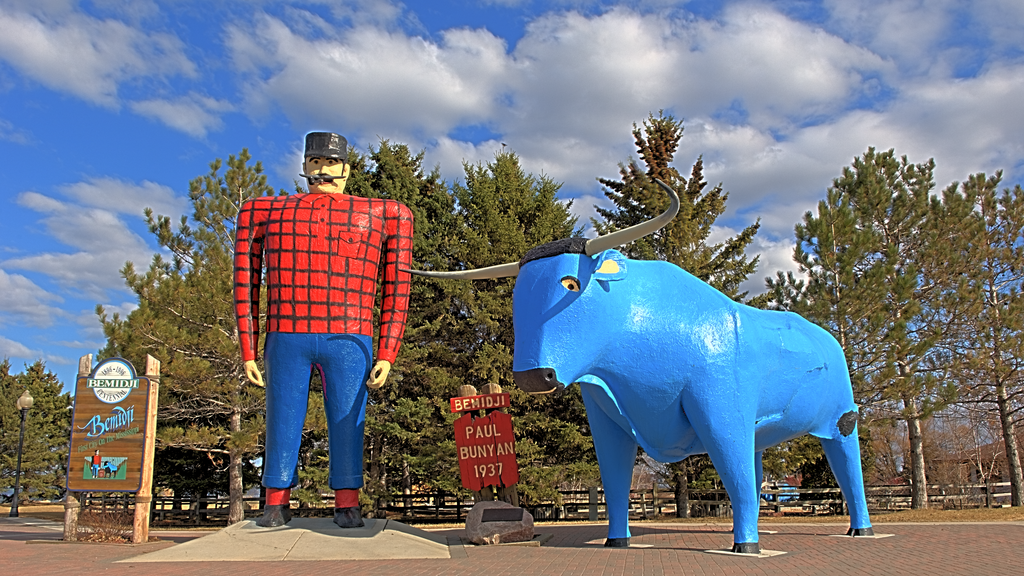
\includegraphics[width=\textwidth]{figures/chapter5/style_based/PaulBunyan_hdrcandy_v2.png}
    \caption{Version I}
    \label{FigStyle:VerI}
\end{subfigure}\hfill
\begin{subfigure}[b]{0.40\textwidth}
    \centering
    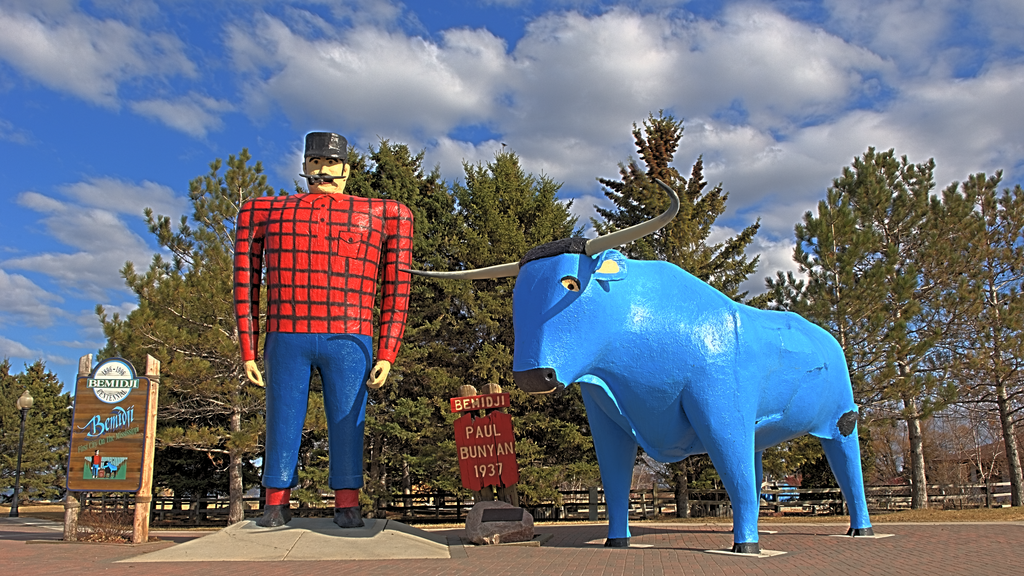
\includegraphics[width=\textwidth]{figures/chapter5/style_based/PaulBunyan_hdrcandy_w0_1.png}
    \caption{$w_0 = 1$, $w_1 = w_2 = 0$}
    \label{FigStyle:VerIIa}
\end{subfigure}\hfill
\begin{subfigure}[b]{0.40\textwidth}
    \centering
    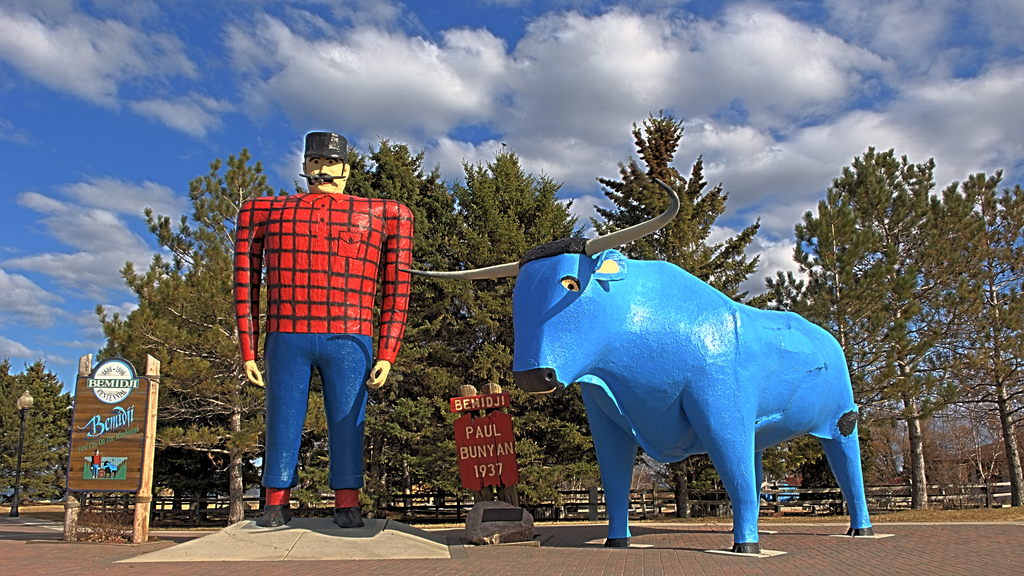
\includegraphics[width=\textwidth]{figures/chapter5/style_based/PaulBunyan_hdrcandy_w0_w1_w2.png}
    \caption{$w_0 = w_1 = w_2 = \frac{1}{3}$}
    \label{FigStyle:VerIIb}
\end{subfigure}\\
\begin{subfigure}[b]{0.40\textwidth}
    \centering
    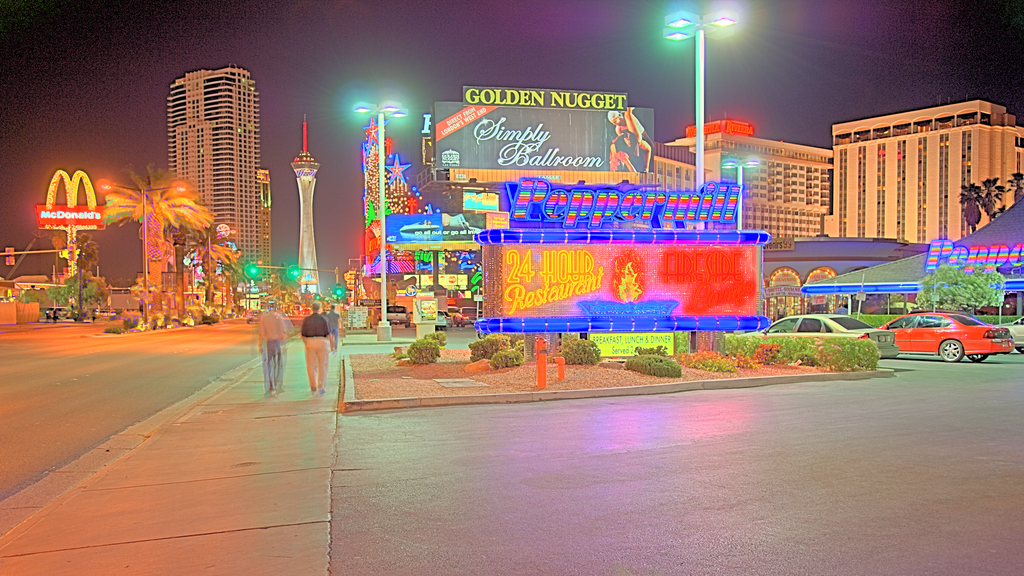
\includegraphics[width=\textwidth]{figures/chapter5/style_based/Peppermill_hdrcandy_v1.png}
    \caption{Original}
    \label{FigStyle:original}
\end{subfigure}\hfill
\begin{subfigure}[b]{0.40\textwidth}
    \centering
    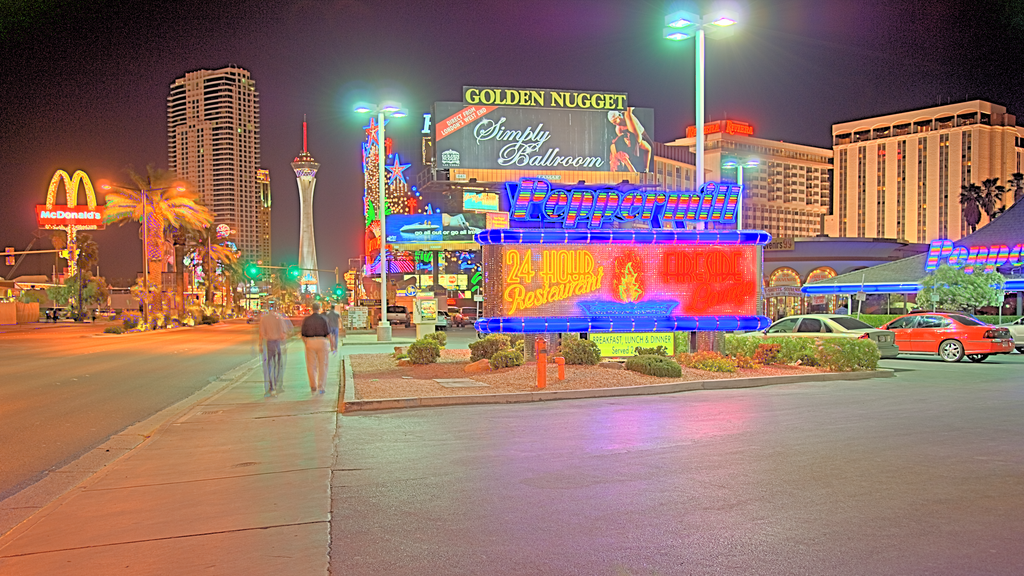
\includegraphics[width=\textwidth]{figures/chapter5/style_based/Peppermill_hdrcandy_v2.png}
    \caption{Version I}
    \label{FigStyle:VerI}
\end{subfigure}\hfill
\begin{subfigure}[b]{0.40\textwidth}
    \centering
    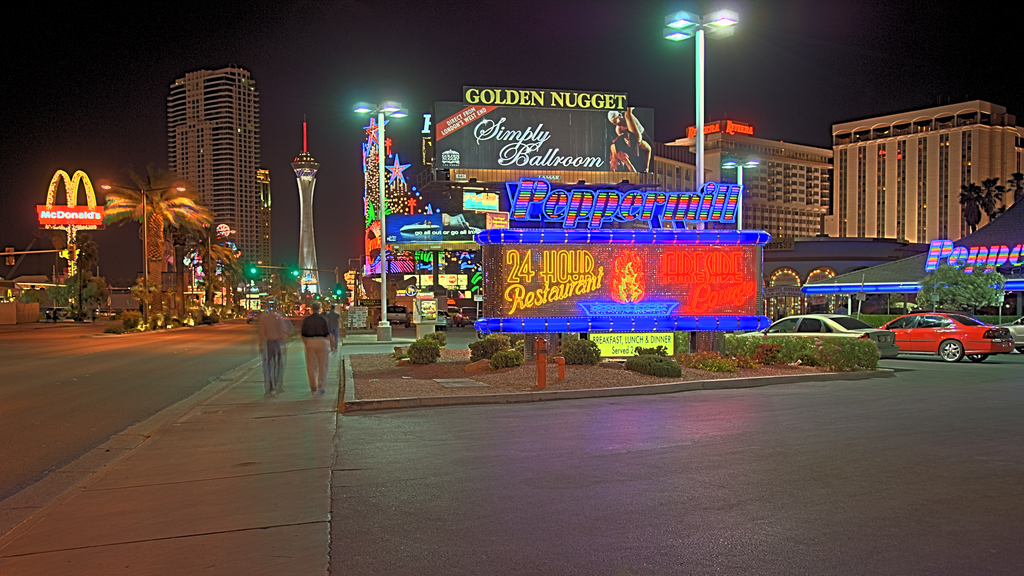
\includegraphics[width=\textwidth]{figures/chapter5/style_based/Peppermill_hdrcandy_w0_1.png}
    \caption{$w_0 = 1$, $w_1 = w_2 = 0$}
    \label{FigStyle:VerIIa}
\end{subfigure}\hfill
\begin{subfigure}[b]{0.40\textwidth}
    \centering
    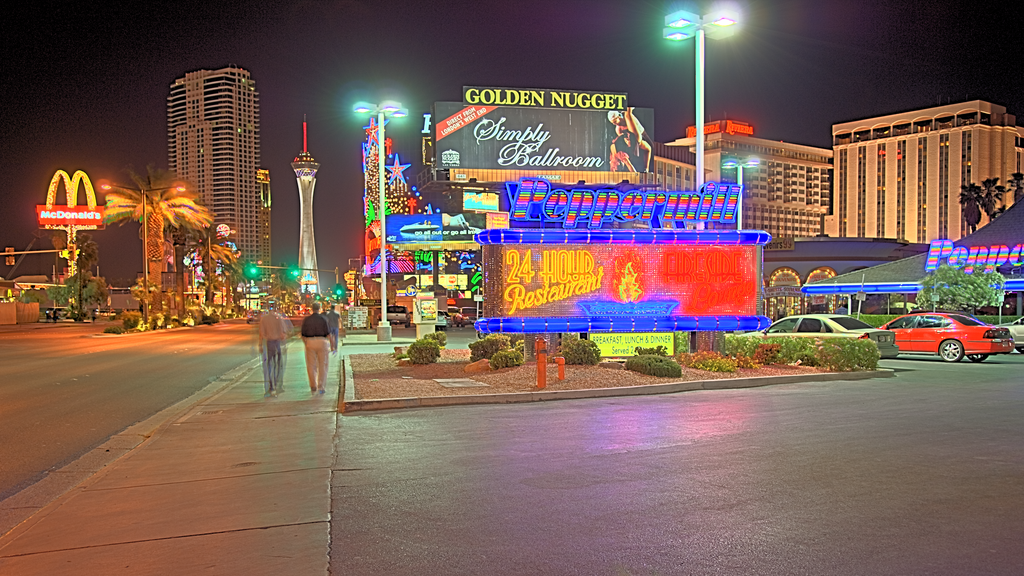
\includegraphics[width=\textwidth]{figures/chapter5/style_based/Peppermill_hdrcandy_w0_w1_w2.png}
    \caption{$w_0 = w_1 = w_2 = \frac{1}{3}$}
    \label{FigStyle:VerIIb}
\end{subfigure}\hfill
\caption{Application of our findings for the style-based tone mapping
    problem.  Original results are shown in the first column, followed
        by Version I in the second column and two variants of Version II
in the last two columns.}
\label{FigStyle}
\end{figure}
\end{landscape}
\chapter{Improved Style-based Tone Mapping}
\label{chp:b6}

Although style based tone mapping has achieved some success for consistently tone mapping different images, the image similarity method given in Section \ref{sec:operation} can be improved with the findings from the conducted user study. In this chapter, two modifications of this method that are made possible by the experimental findings of the user study is given. The first technique uses all of the image features utilized in Chapter~\ref{chp:b5} with different weights to estimate tone mapping parameters in the operation phase. Meanwhile, the second technique relates tone mapping parameters and image features for the estimation.

\section{Parameter Interpolation with All Features}
\label{sec:all_features}

In the first modification, the model features given in Table \ref{tab:table_feature} are extracted from the selected HDR image and calibration images. Then, the distances between these features are calculated separately using the corresponding distance metrics given in the same table. After that, the weighted average of these feature distances are calculated. The weights used are the coefficients of the logistic regression model (Equation \ref{eq:log_regression}) obtained from the user experiment, with the idea that less important features should also contribute less to the distance. This operation can be summarized with the following equation:

\begin{equation}
    d_i = \sum_{j=1}^{6}c_j d_j(\mathbf{f_i}, \mathbf{f_{ij}})
\end{equation}

where $c_j$ is the coefficient of the $j^{th}$ feature, $\mathbf{f_j}$ is the $j^{th}$ feature of the input image, $\mathbf{f_{ij}}$ is the same for the $i^{th}$ calibration image, and finally $d_j$ is the distance metric for the $j^{th}$ feature. The result $d_i$ represents the combined distance between the input image and the corresponding calibration image. These combined distances are calculated between the selected HDR image and all calibration images. The tone mapping parameters for the selected HDR image are then interpolated using inverse distance transform as in Equation \ref{eq:inv_distance_transform}. This method differs from the initially presented approach in several aspects: 

\begin{itemize}
    \item Using a different and more representative set of features, luminance which is one of the most important features of HDR images has a separate feature vector,
    \item More suitable distance metrics for feature types, for example, EMD takes into account bin proximity for calculating differences between histograms,
    \item Instead of using a single fused feature vector, each feature distance calculated separately,
    \item Employing a weighted average of feature vector distances with weights obtained from a user experiment, compared to using equal weight.
\end{itemize}

In Figure~\ref{fig:algo_updated}, the modified style-based tone mapping algorithm is shown. Note that while the calibration phase has not changed, the operation phase has been adjusted with the changes listed above compared to the initial version of the algorithm given in Figure~\ref{fig:calibration_operation}. 

\begin{figure}
    \centering
    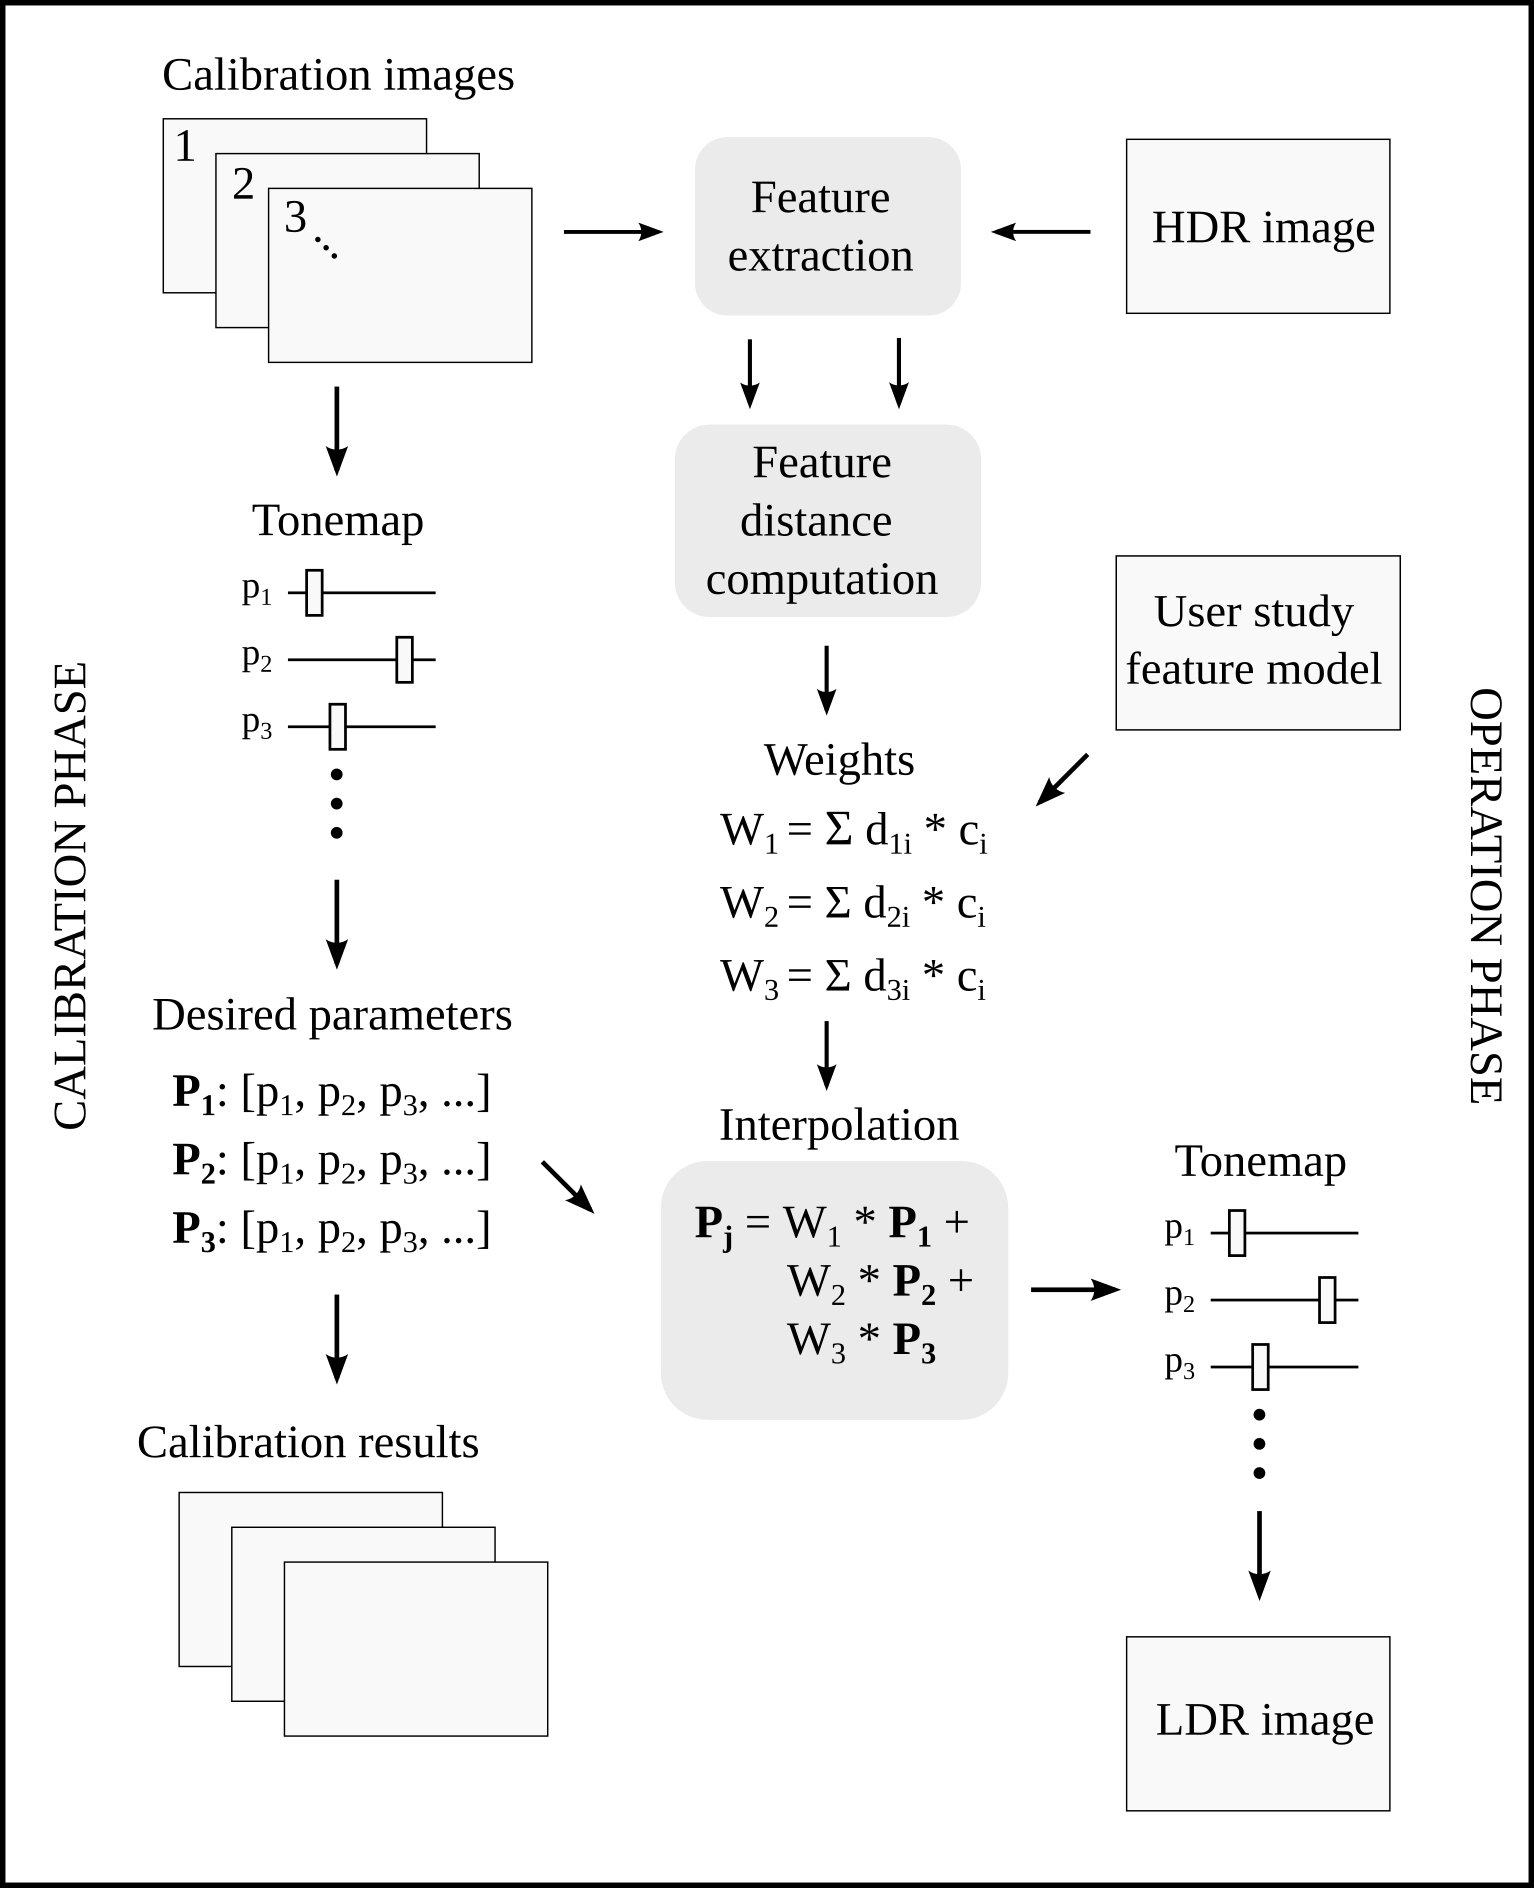
\includegraphics[width=\textwidth]{figures/algorithm_updated.png}
    \caption{Modified style-based tone mapping algorithm with the findings of the user experiment. Compared to the initial method given in Figure~\ref{fig:calibration_operation}, more representative set of features are extracted and distances between these features are computed separately. Besides, instead of using equal weights on feature distances, the weights estimated from user study are employed.}
    \label{fig:algo_updated}
\end{figure}

\section{Parameter Interpolation with Related Features}
\label{sec:related_features}
While the previous approach calculates a single distance value between the given image and calibration images and use this value to interpolate all tone mapping parameters, the second modification described in this section relates the model features with the tone mapping parameters and interpolates individual tone mapping parameters with different weights. In order to achieve this, the relationships defined in Table~\ref{tab:feature_mapping} are used.

\begin{table}
\caption{Model features used for interpolation of tone mapping parameters.}
\centering
\begin{tabular}{l | l}
\label{tab:feature_mapping}
\textbf{Tone mapping parameter} & \textbf{Model feature}\\
\hline
Brightness ($t_b$) & Luminance \\
Contrast ($t_c$) & Luminance \\
Black point ($t_{bp}$) & Luminance \\
White point ($t_{wp}$) & Luminance \\
Color saturation ($t_s$) & Color \\
Small detail strength ($t_{\lambda_s}$) & Texture \\
Medium detail strength ($t_{\lambda_m}$ ) & Texture \\
Large detail strength ($t_{\lambda_l}$) & Texture
\end{tabular}
\end{table}


As an example, the brightness parameter $t_b$ is computed by interpolating the $t_{b_i}$ parameters of the calibration images by using the similarity between the luminance features:

\begin{equation}
   t_b = { {\sum_{i=1}^N { {1} \over {d_{lum} (lum, lum_i)} } t_{b_i} } \over {\sum_{i=1}^N} { {1} \over {d_{lum} (lum, lum_i)} } }
\end{equation}

Other tone mapping parameters that are related to the model features are interpolated analogously. Because GIST and deep learning features are not directly linked to a specific appearance phenomenon but are measures of overall similarity between the given images, they are not directly linked to specific tone mapping parameters. Instead these features are experimented with merging them using the individually interpolated parameters as follows: 

\begin{equation}
   \mathbf{t} = w_0\mathbf{t_0} + w_1\mathbf{t_1} + w_2\mathbf{t_2}, 
\end{equation}

where $\mathbf{t_0}$ represents individually interpolated TMO parameters (given in Table~\ref{tab:feature_mapping}), $\mathbf{t_1}$ TMO parameters interpolated as a whole using GIST similarity only, and $\mathbf{t_2}$ TMO parameters interpolated as a whole using solely deep learning feature similarity. The weights control the influence of TMO parameters that are computed by using these different approaches.

\section{Results}
In Figure~\ref{FigStyle}, several results are compared that obtained by using the initial style based tone mapping method as well as with the two modifications proposed in the previous sections, Section~\ref{sec:related_features} and Section~\ref{sec:all_features}. 

In the first row of the figure, the tone mapping results of the ``Paul Bunyan'' scene from the HDR Photographic Survey~\cite{fairchild2007hdr} is shown. This scene depicts a bright outdoors environment with colorful foreground objects. It may be noted that all results are similar but the individual parameter interpolation with equally weighted GIST and deep learning features (d) has slightly higher contrast (please refer to Appendix~\ref{app:results} with high resolution images for better comparison). The overall \emph{candy} style is preserved in all images. 

In the second row of the figure, ``Peppermill'' night scene from the same dataset is shown. This is a night scene of a street with some bright lights and banners. For this scene the difference of the second modification, parameter interpolation with related features, is more clear as images in (c) and (d) exhibit a darker rendering, which is more suitable for a night scene. The reason for this darkening effect is that the brightness parameter, $t_b$, for tone mapping becomes more similar to the $t_b$ parameter of the night image in the calibration images due to the similarity of the \emph{luminance} features between these images. The addition of GIST and deep learning features with equal weight in (d) yields a slightly brighter image compared to (c). Similar to the results of the previous image overall \emph{candy} style is preserved also in this image. Appendix~\ref{app:results} has higher resolution versions of the results for more clear observation of the differences.


\afterpage{
\begin{landscape}
\begin{figure}
\begin{subfigure}[b]{0.40\textwidth}
    \centering
    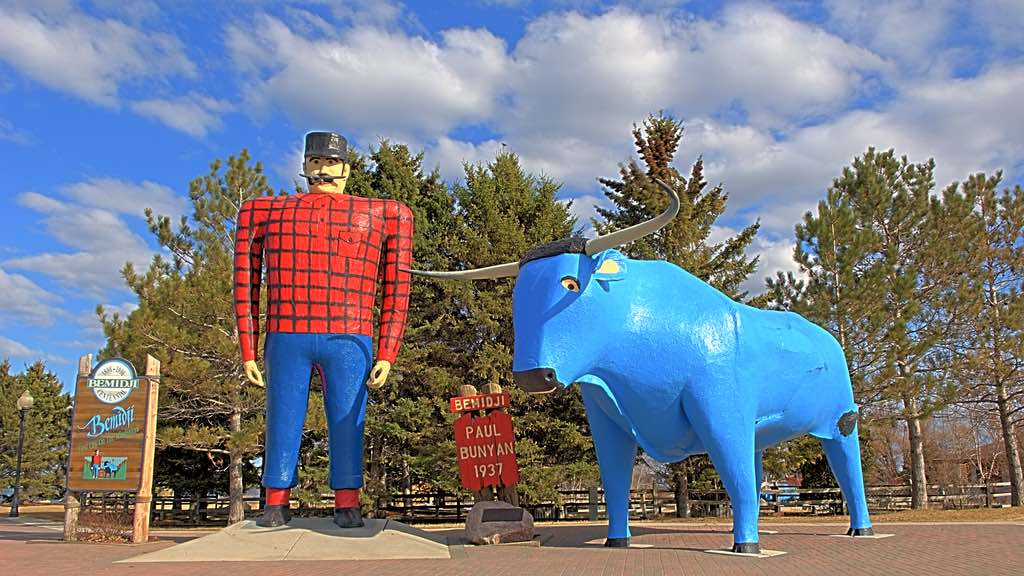
\includegraphics[width=\textwidth]{figures/chapter5/style_based/PaulBunyan_hdrcandy_v1_small.jpg}
    \caption{Initial}
    \label{FigStyle:original_paul_bunyan}
\end{subfigure}\hfill
\begin{subfigure}[b]{0.40\textwidth}
    \centering
    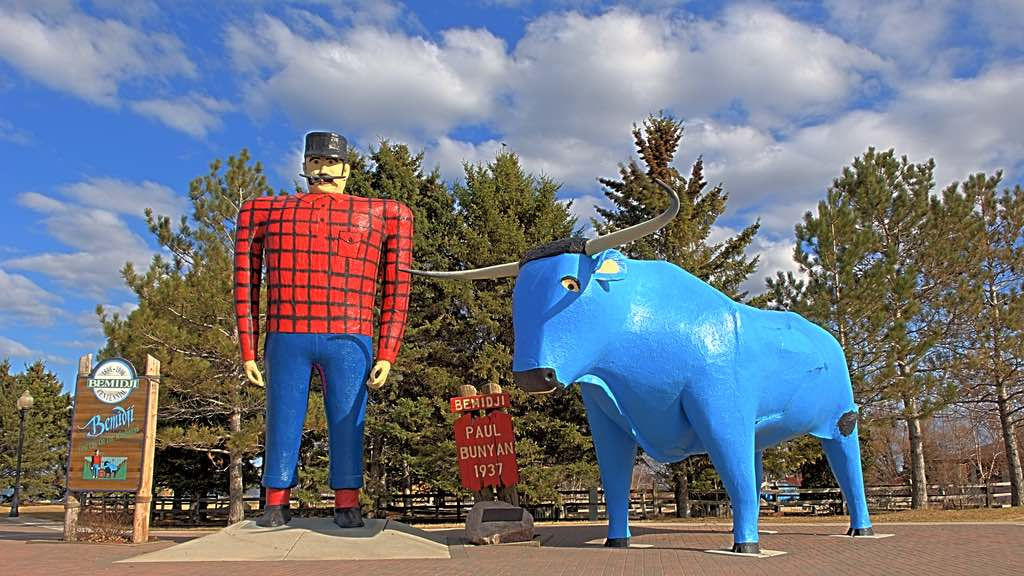
\includegraphics[width=\textwidth]{figures/chapter5/style_based/PaulBunyan_hdrcandy_v2_small.jpg}
    \caption{Version I}
    \label{FigStyle:VerI_paul_bunyan}
\end{subfigure}\hfill
\begin{subfigure}[b]{0.40\textwidth}
    \centering
    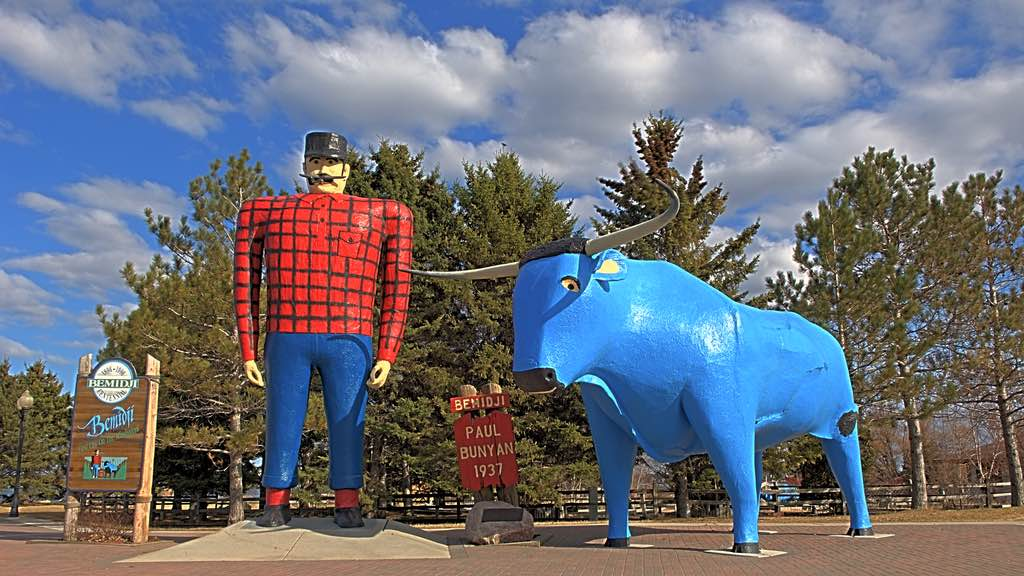
\includegraphics[width=\textwidth]{figures/chapter5/style_based/PaulBunyan_hdrcandy_w0_1_small.jpg}
    \caption{$w_0 = 1$, $w_1 = w_2 = 0$}
    \label{FigStyle:VerIIa_paul_bunyan}
\end{subfigure}\hfill
\begin{subfigure}[b]{0.40\textwidth}
   \centering
    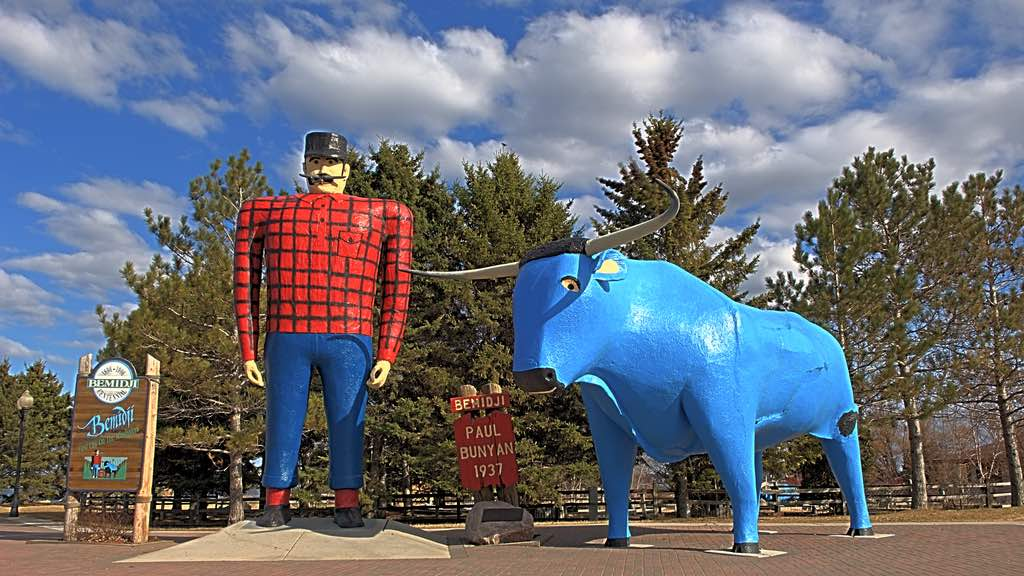
\includegraphics[width=\textwidth]{figures/chapter5/style_based/PaulBunyan_hdrcandy_w0_w1_w2_small.jpg}
    \caption{$w_0 = w_1 = w_2 = \frac{1}{3}$}
    \label{FigStyle:VerIIb_paul_bunyan}
\end{subfigure}\\
\begin{subfigure}[b]{0.40\textwidth}
    \centering
    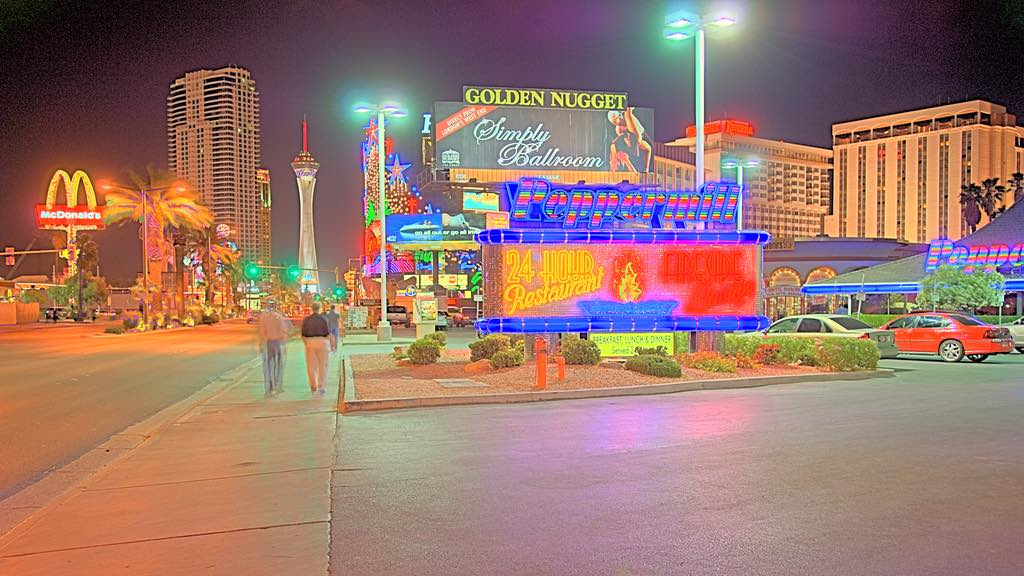
\includegraphics[width=\textwidth]{figures/chapter5/style_based/Peppermill_hdrcandy_v1_small.jpg}
    \caption{Initial}
    \label{FigStyle:original_peppermill}
\end{subfigure}\hfill
\begin{subfigure}[b]{0.40\textwidth}
    \centering
    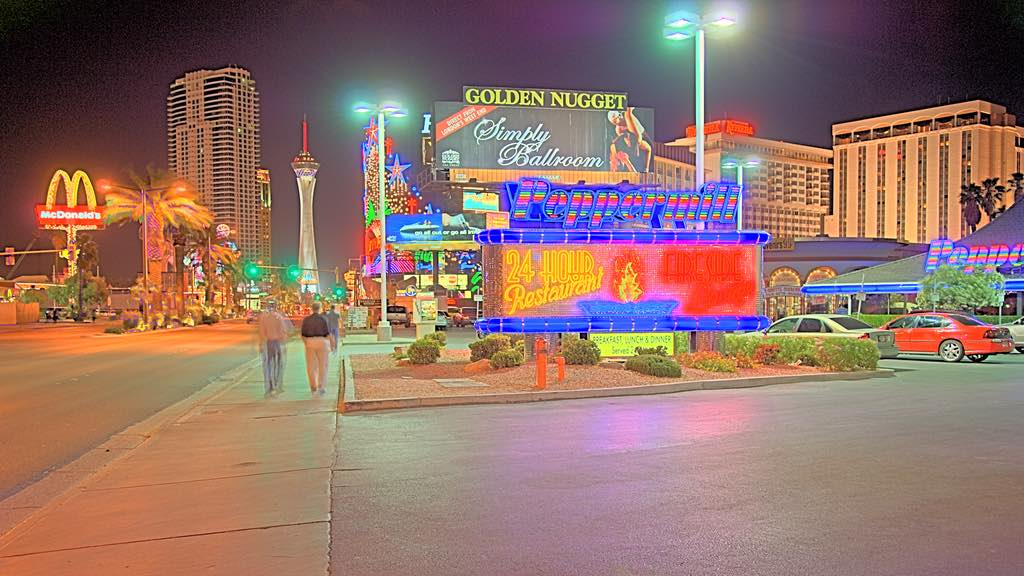
\includegraphics[width=\textwidth]{figures/chapter5/style_based/Peppermill_hdrcandy_v2_small.jpg}
    \caption{Version I}
    \label{FigStyle:VerI_peppermill}
\end{subfigure}\hfill
\begin{subfigure}[b]{0.40\textwidth}
    \centering
    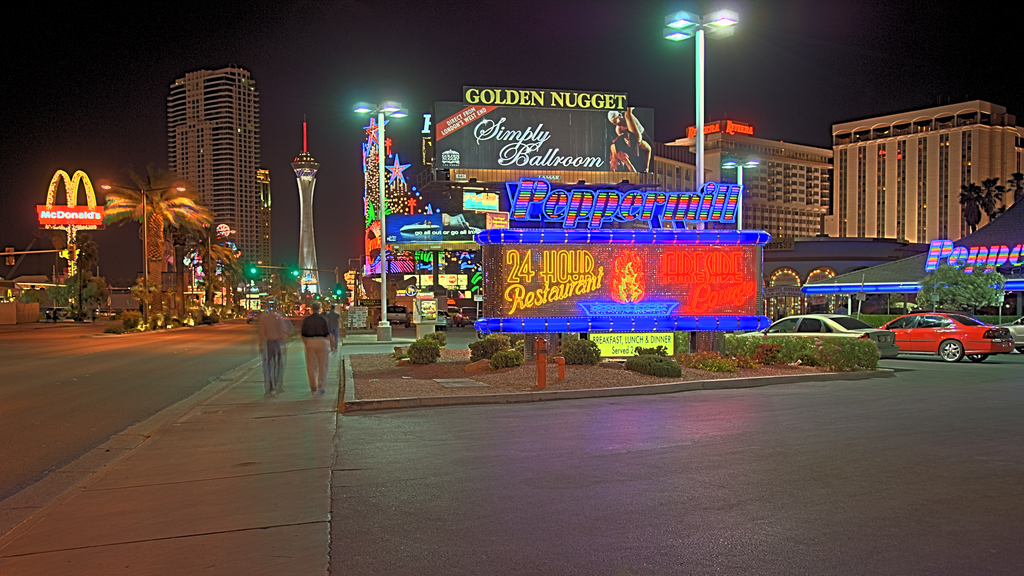
\includegraphics[width=\textwidth]{figures/chapter5/style_based/Peppermill_hdrcandy_w0_1.png}
    \caption{$w_0 = 1$, $w_1 = w_2 = 0$}
   \label{FigStyle:VerIIa_peppermill}
\end{subfigure}\hfill
\begin{subfigure}[b]{0.40\textwidth}
    \centering
    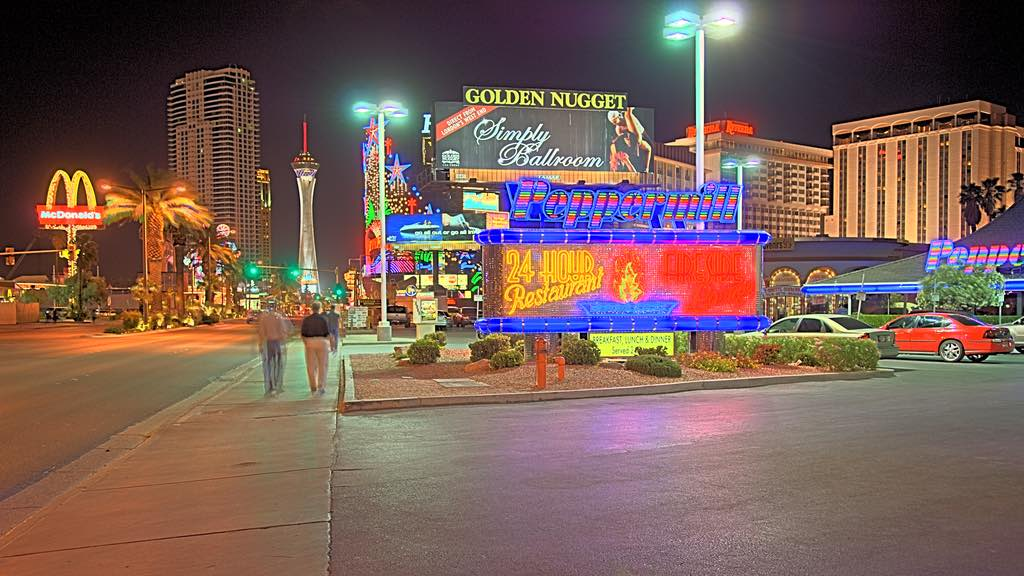
\includegraphics[width=\textwidth]{figures/chapter5/style_based/Peppermill_hdrcandy_w0_w1_w2_small.jpg}
    \caption{$w_0 = w_1 = w_2 = \frac{1}{3}$}
    \label{FigStyle:VerIIb_peppermill}
\end{subfigure}\hfill
\caption{Application of the user study findings for the style-based tone mapping
    problem.  Initial results are shown in the first column, followed
        by Version I in the second column and two variants of Version II
in the last two columns.}
\label{FigStyle}
\end{figure}
\end{landscape}}


\bibliographystyle{ieeetr} 
\bibliography{references} 

%
% References in Bibtex format goes into below indicated file with .bib extension
%\bibliography{thesis_references}
% You can use full name of authors, however most likely some of the Bibtex entries you will find, will use abbreviated first names
% If you don't want to correct each of them by hand, you can use abbreviated style for all of the references

%\bibliographystyle{abbrv}

% if you have more that one appendix, then use \appendices, otherwise use 
% \appendix
% \appendix
\chapter{Clusters of the Hdr Image Dataset}
\label{app:clusters}

\begin{figure}[h!]
\begin{center}
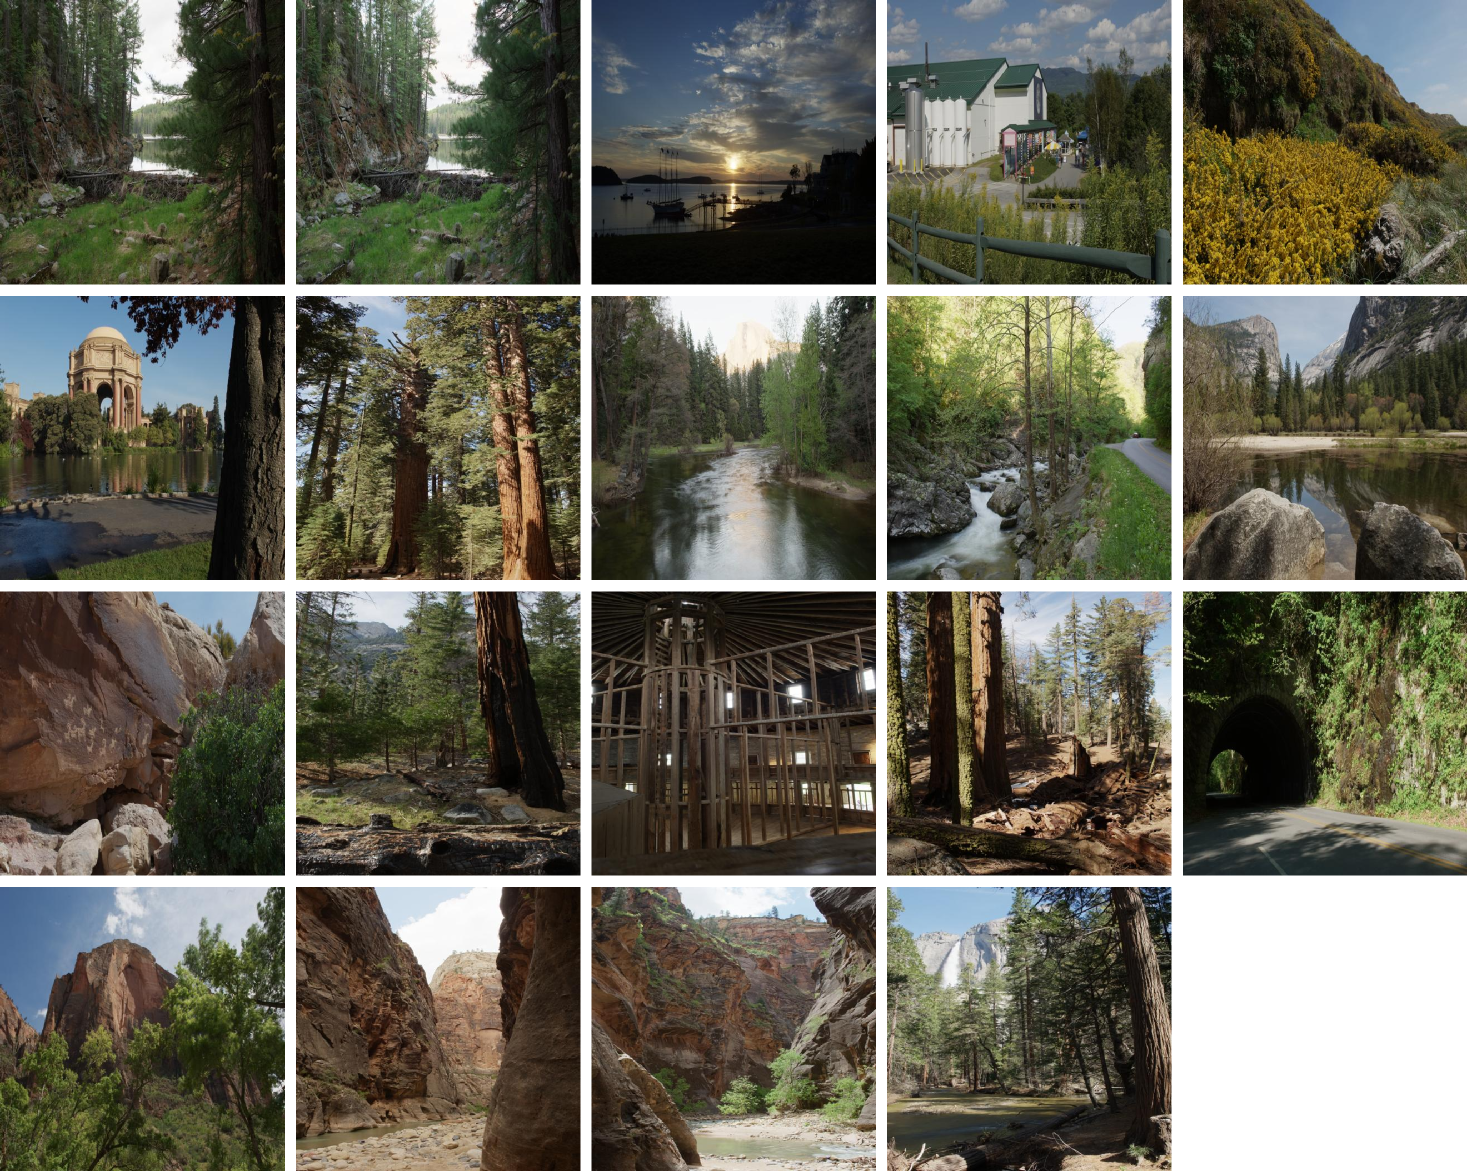
\includegraphics[width=\textwidth]{appendix1/cluster1.png}
\caption{Cluster I, clustering result of Fairchild's HDR Dataset~\cite{fairchild2007hdr} for calibration image selection.}
\end{center}
\end{figure}

\begin{figure}
\begin{center}
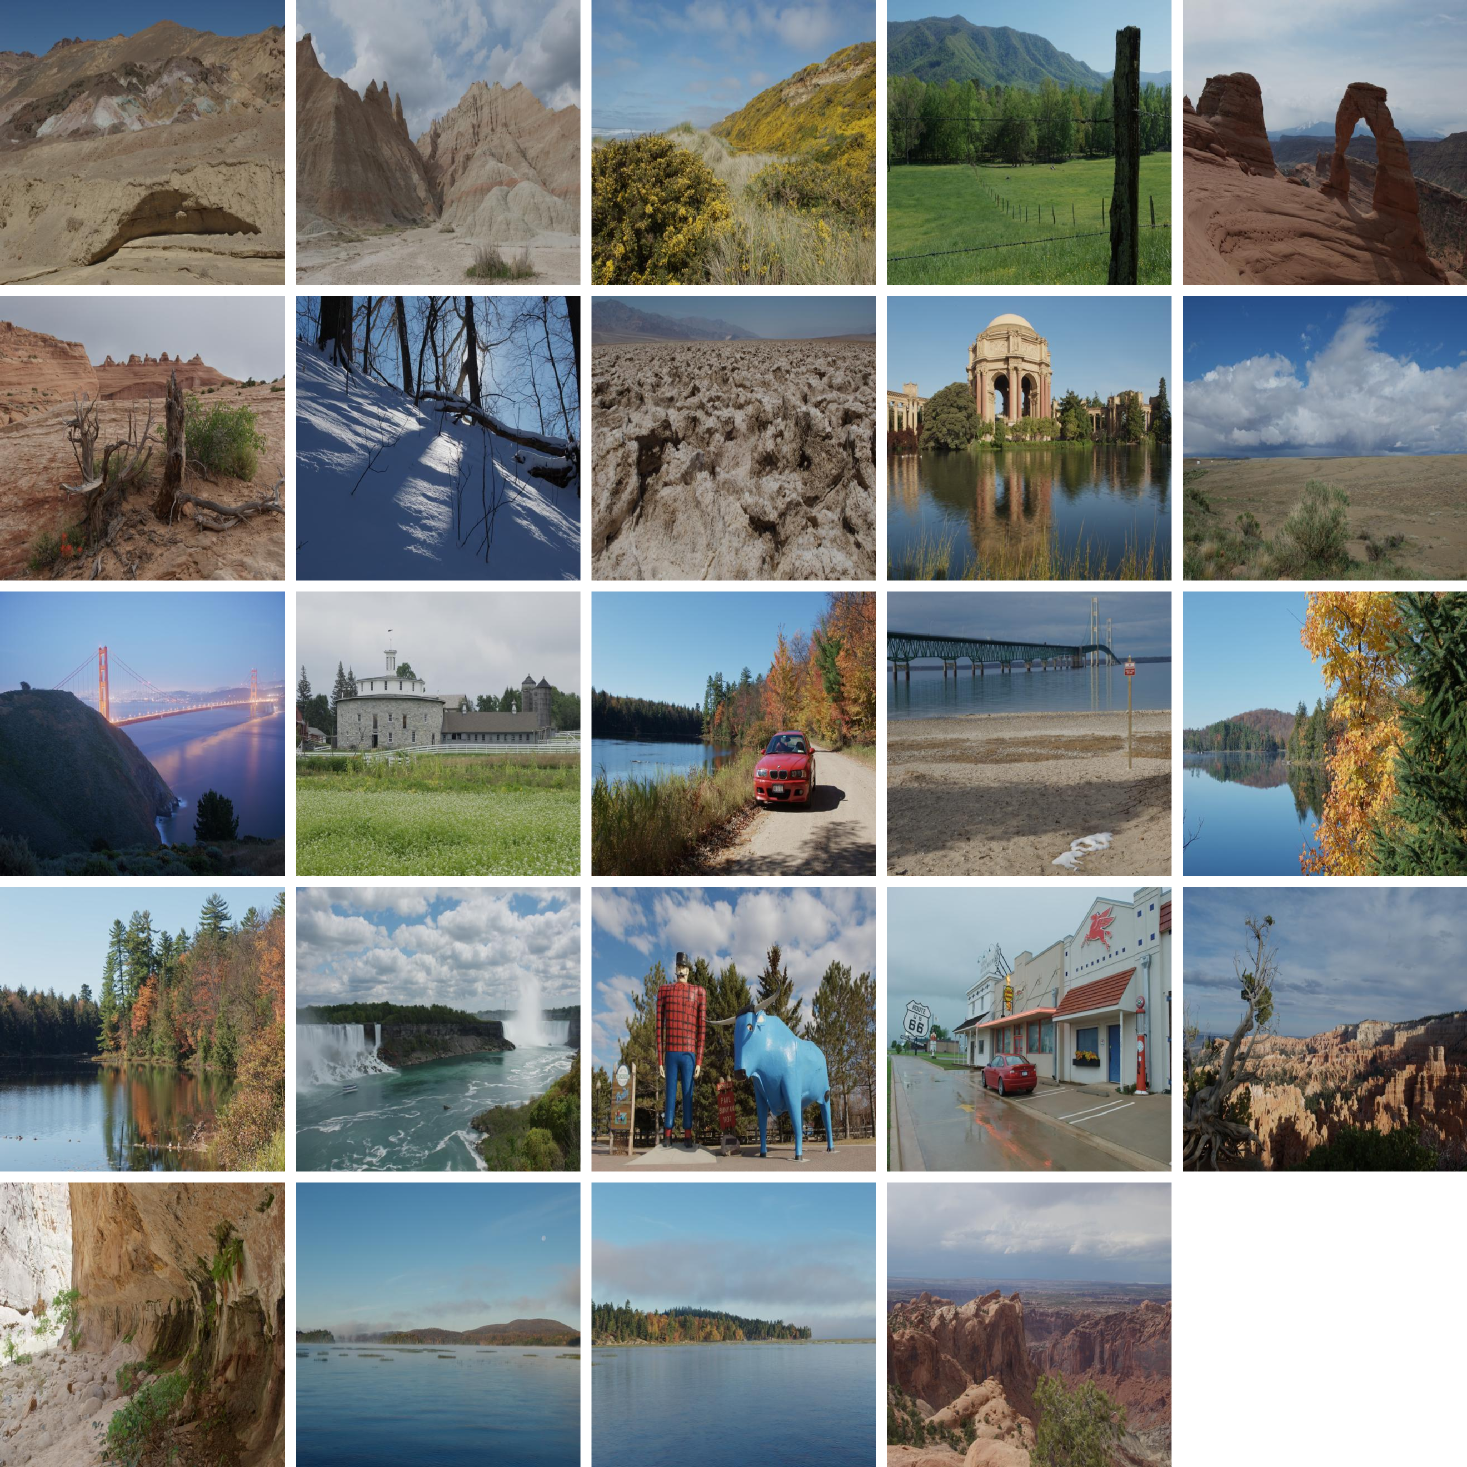
\includegraphics[width=\textwidth]{appendix1/cluster2.png}
\caption{Cluster II, clustering result of Fairchild's HDR Dataset~\cite{fairchild2007hdr} for calibration image selection.}
\end{center}
\end{figure}

\begin{figure}
\begin{center}
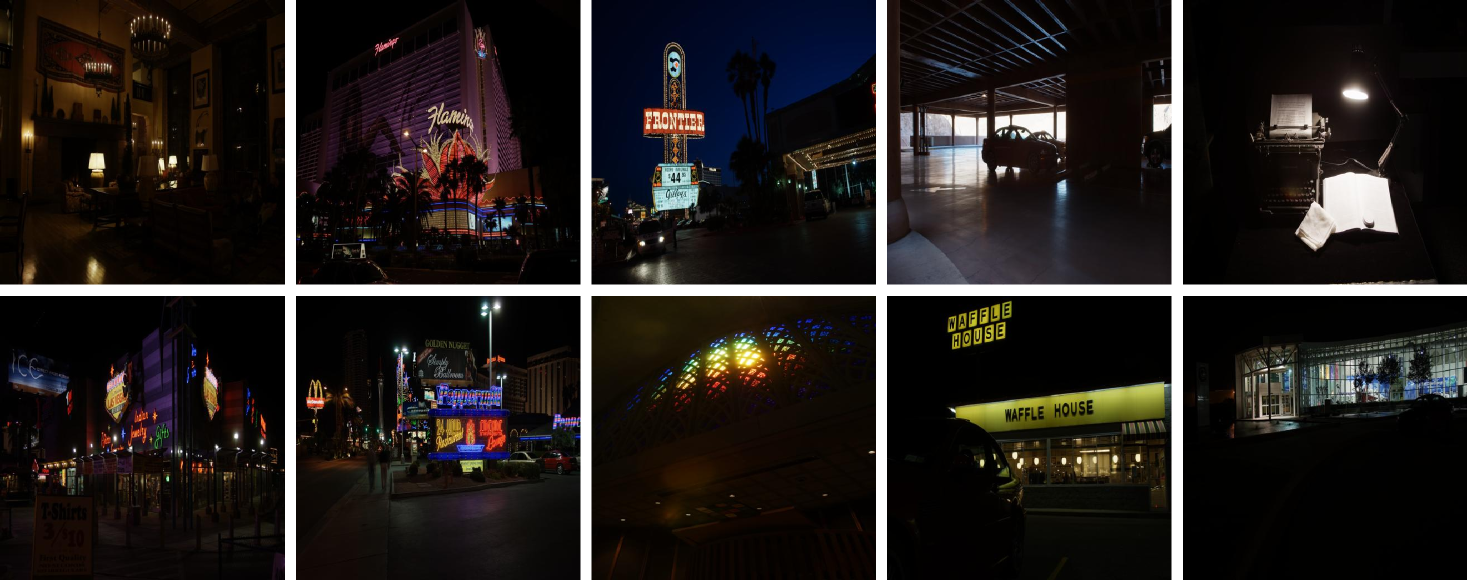
\includegraphics[width=\textwidth]{appendix1/cluster3.png}
\caption{Cluster III, clustering result of Fairchild's HDR Dataset~\cite{fairchild2007hdr} for calibration image selection.}
\end{center}
\end{figure}

\begin{figure}
\begin{center}
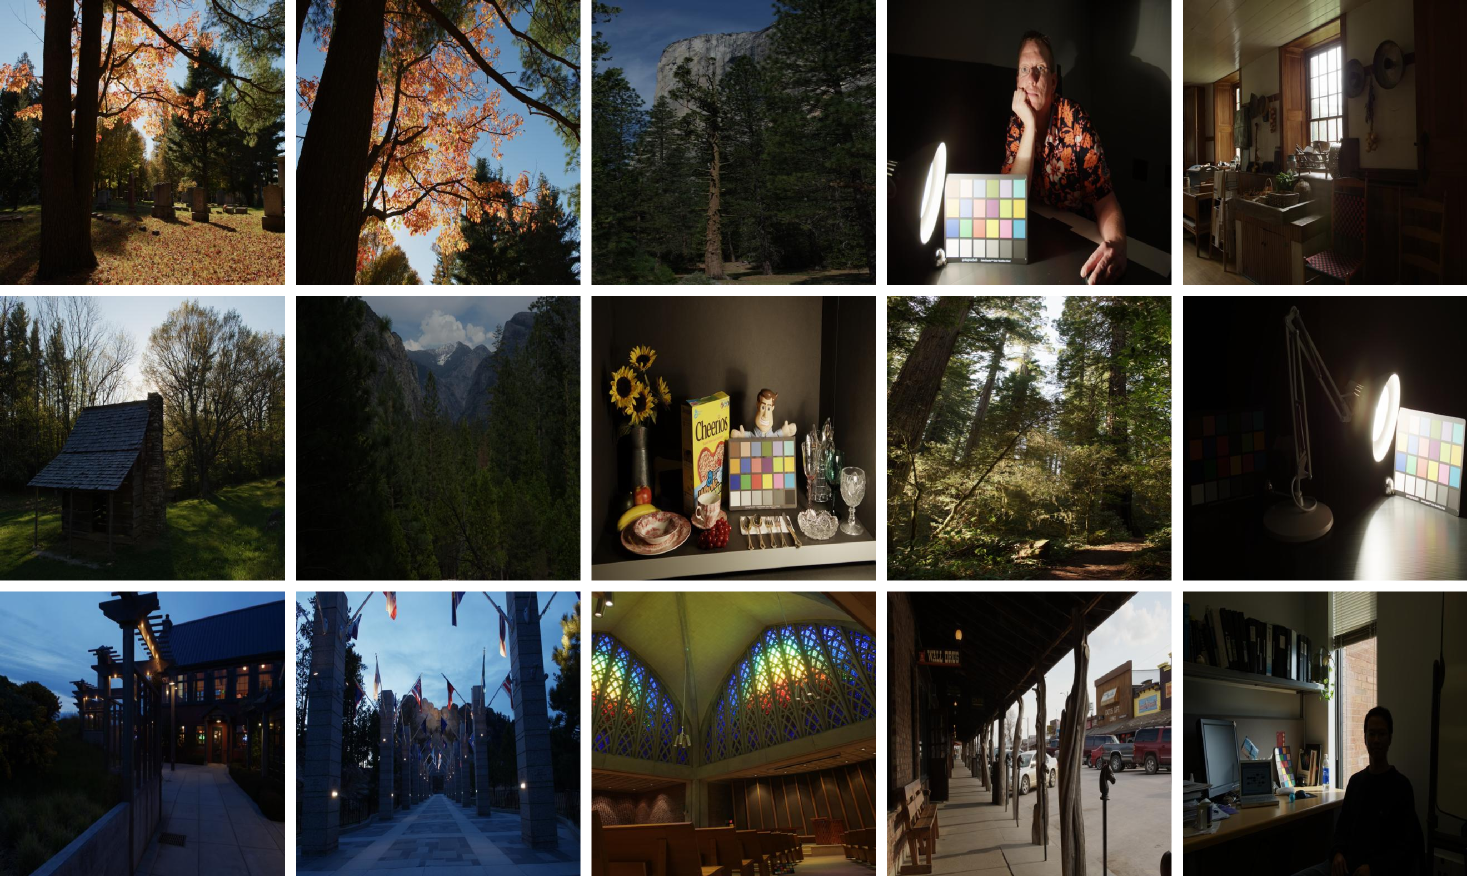
\includegraphics[width=\textwidth]{appendix1/cluster4.png}
\caption{Cluster IV, clustering result of Fairchild's HDR Dataset~\cite{fairchild2007hdr} for calibration image selection.}
\end{center}
\end{figure}

\begin{figure}
\begin{center}
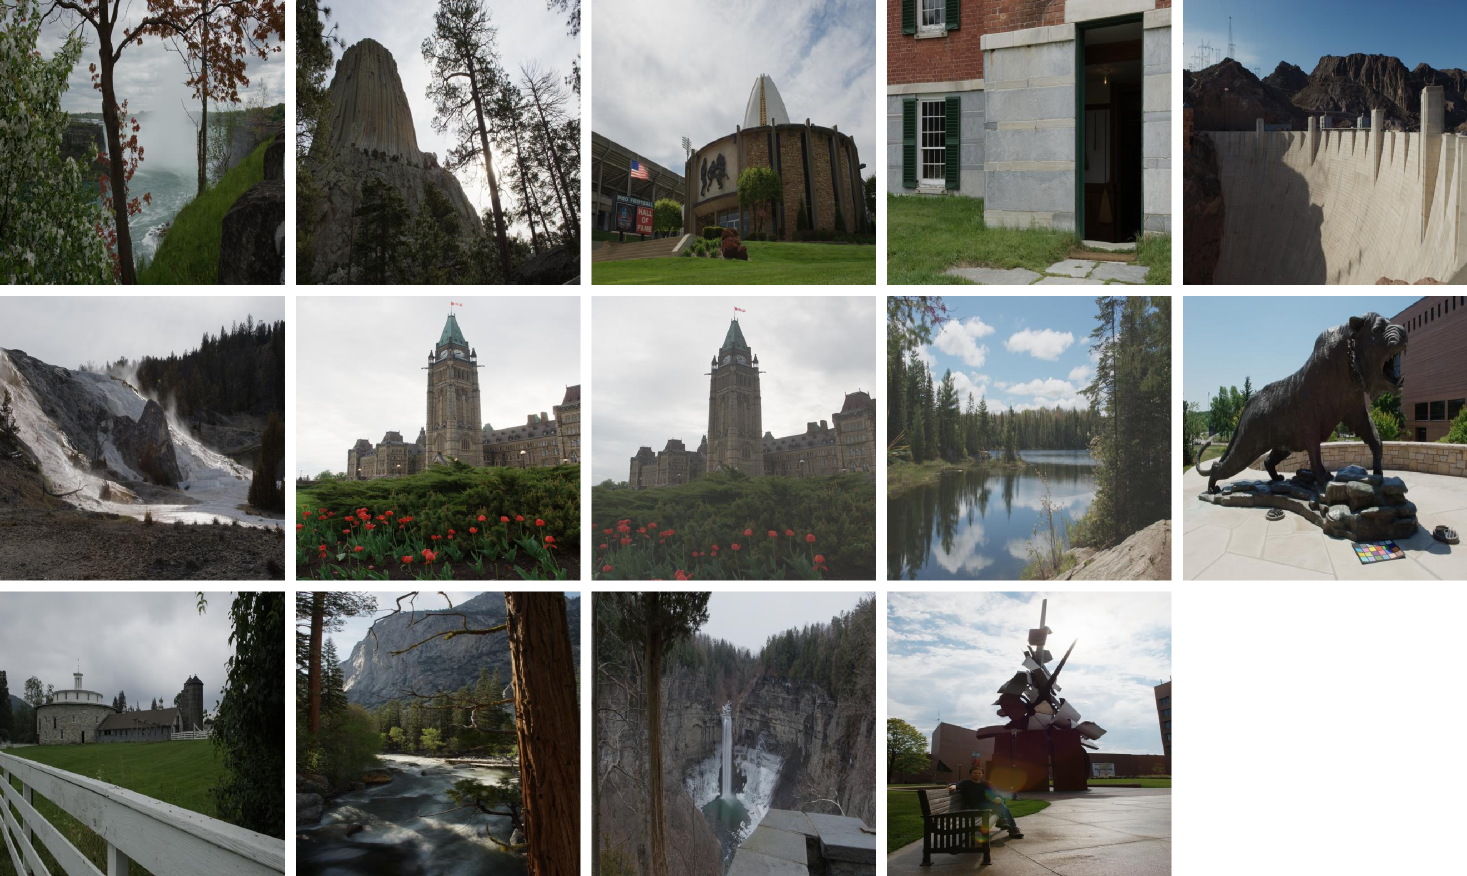
\includegraphics[width=\textwidth]{appendix1/cluster5.png}
\caption{Cluster V, clustering result of Fairchild's HDR Dataset~\cite{fairchild2007hdr} for calibration image selection.}
\end{center}
\end{figure}

\begin{figure}
\begin{center}
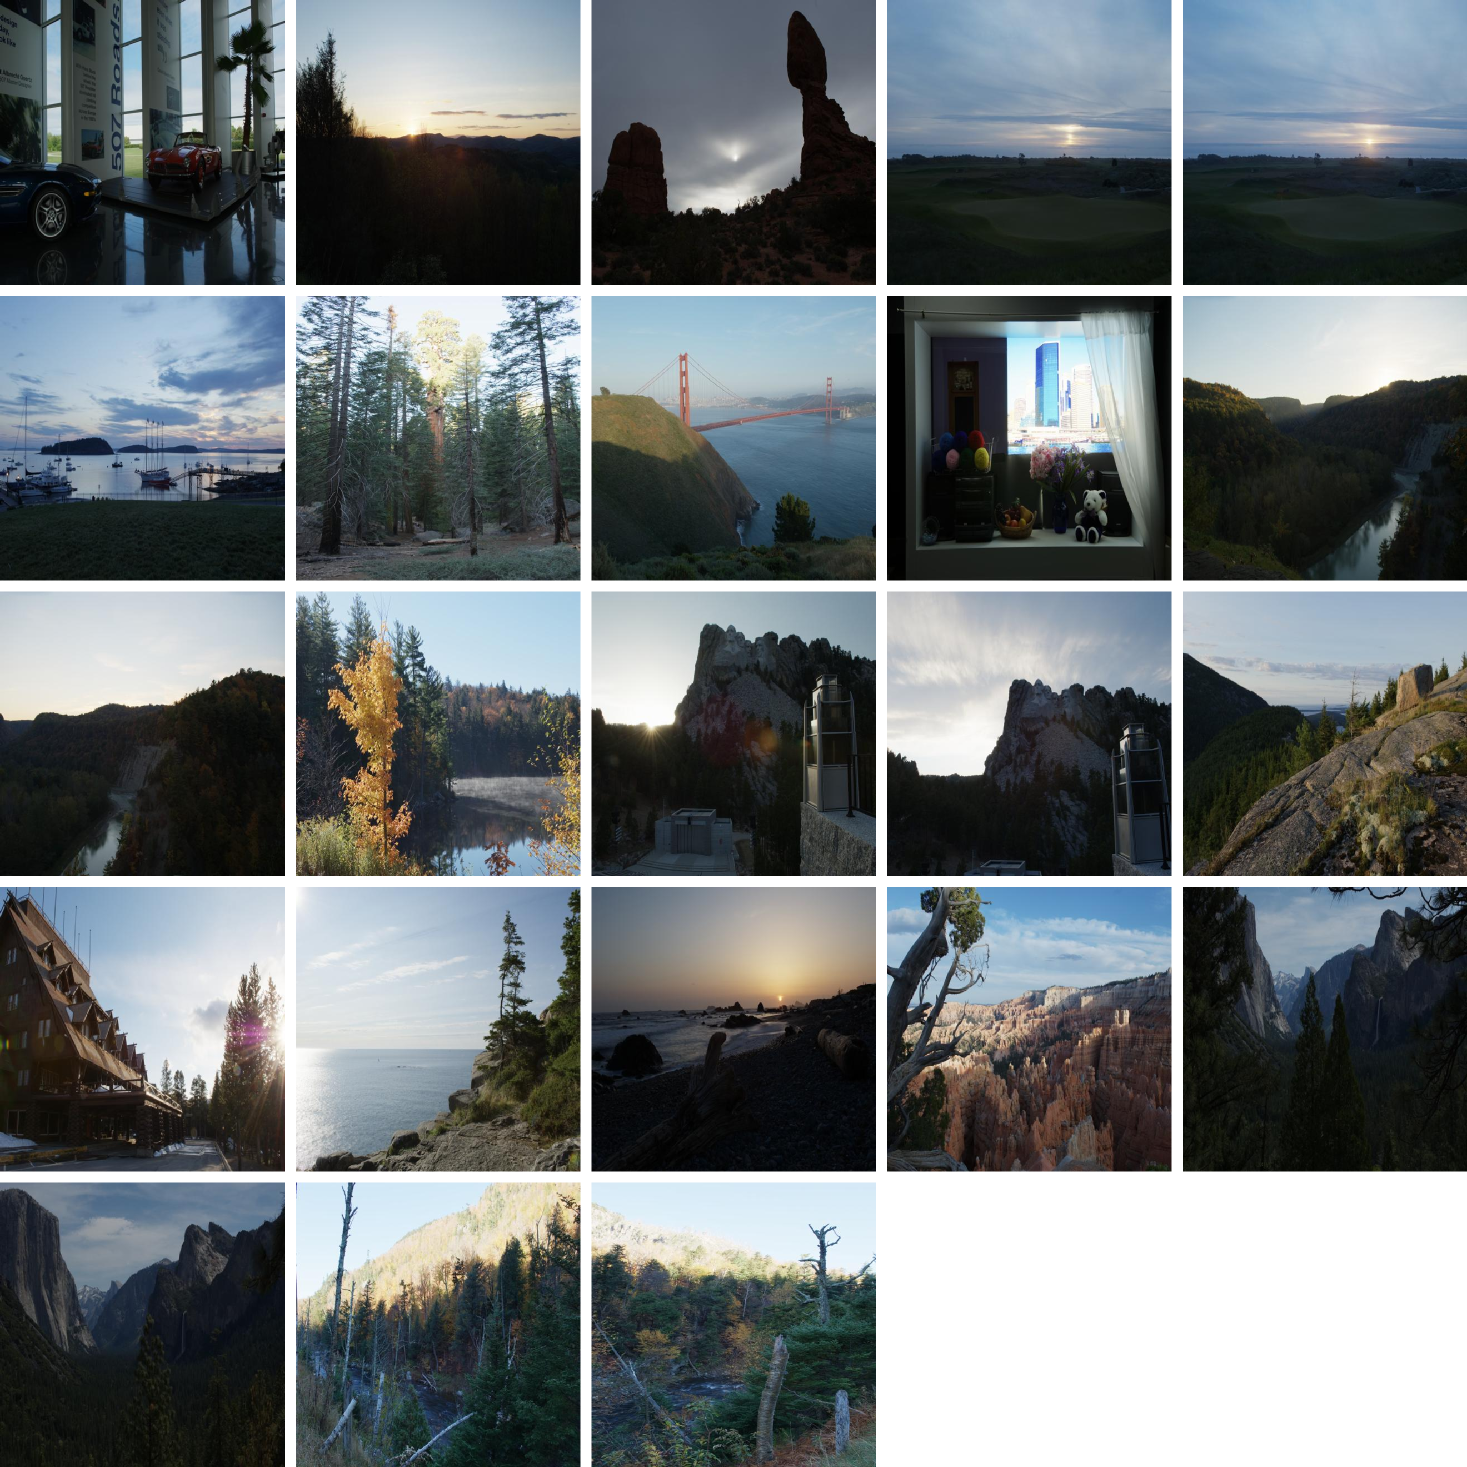
\includegraphics[width=\textwidth]{appendix1/cluster6.png}
\caption{Cluster VI, clustering result of Fairchild's HDR Dataset~\cite{fairchild2007hdr} for calibration image selection.}
\end{center}
\end{figure}
\end{document}
